%! Author = lazza
%! Date = 10/04/2022

% Preamble
\documentclass[9pt, twocolumn, twoside]{article}

% Packages
\usepackage[a4paper, total={7in, 10in}]{geometry}
\usepackage{amsmath}
\usepackage{graphicx}
\usepackage{textcomp}
\usepackage[utf8]{inputenc}
\usepackage[T1]{fontenc}
\usepackage{enumitem}
\usepackage{booktabs}
\usepackage{bitset}
\usepackage{xcolor}
\usepackage{color}
\usepackage{intcalc}
\usepackage{float}
\usepackage{amsfonts}
\usepackage{wasysym}
\usepackage{adjustbox}
\usepackage{biblatex}
%\usepackage{latexsymb}

\title{Advanced Computer Architectures \\ \large Professor Marco D. Santambrogio}
%\author{Gabriele Lazzarelli}
\date{Spring 2022}

\begin{document}
    \maketitle
    \noindent\makebox[\textwidth]{
\includegraphics[width=5cm]{images/LogoPolimi}}
    \vfill
    \noindent\makebox[\textwidth]{github.com/glazzarelli/ACA-notes}

    \clearpage
    \tableofcontents
    \clearpage

    \setlist{topsep=4pt,itemsep=1pt,partopsep=2pt, parsep=2pt}
    %! Author = lazza
%! Date = 10/04/2022

% Preamble
\documentclass[11pt]{article}

% Packages
\usepackage{amsmath}

% Document
\begin{document}
    \section{Introduction}\label{sec:introduction}


    \subsection{Taxonomy}\label{subsec:taxonomy}

    \subsection{Parallelism}\label{subsec:parallelism}

    \subsubsection{Instruction level}
    \subsubsection{Thread level}
    \subsubsection{Both SMT}
    \subsubsection{Heterogeneous}


    \subsection{Heterogeneous systems}\label{subsec:heterogeneous-systems}



\end{document}
    %! Author = lazza
%! Date = 09/05/2022

\section{Performance and Cost}\label{sec:performance-and-cost}
When we say that one computer is faster than another what do we mean?
It depends on what is important.

Two metrics:
\begin{description}
    \item[Computer system user] minimize elapsed time for program execution:\\
    \textbf{latency:} (response time) execution time = time\_end - time\_start
    \item[Computer center manager] maximize completion rate \(=\frac{\#jobs}{\sec}\)\\
    \textbf{throughput:} total amount of work done in a given time
\end{description}
Throughput \(= \frac{1}{latency}\) only if there is not overlap between instructions, otherwise throughput >
response time.

\subsection{Measures}\label{subsec:measures}
\begin{gather*}
    \text{"X is k\% faster than Y"} = \frac{\text{execution time (y)}}{\text{execution time (x)}} = 1 + \frac{n}{100}\\
    \text{\textbf{Performance (x)}} = \frac{1}{\text{execution time(x)}}\\
    \Rightarrow \text{"X is k\% faster than Y"} = \frac{\text{performance (x)}}{\text{performance (y)}} = 1 +
\frac{n}{100}\\
\end{gather*}

\[\text{\textbf{Speed up (x,y)}} = \frac{\text{performance (x)}}{\text{performance (y)}}\]

\subsection{Amdahl's Law}\label{subsec:amdahl's-law}
Suppose that an enhancement E accelerates a fraction F of the task by a factor S (speedup enhanced), and the remainder
of the task in unaffected.

\begin{figure}[H]
    \centering
    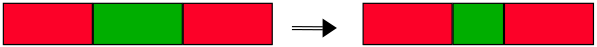
\includegraphics[scale = 0.3]{images/amdahls-law}
    \caption{In green the (F) fraction enhanced.}
    \label{fig:amdalhs-law}
\end{figure}

\begin{gather*}
    ExTime_{new} = ExTime_{old} \times \left( \left( 1 - F_{en} \right) +
\frac{F_{en}}{S_{en}} \right)\\
    \mathbf{S_{overall}} = \frac{ExTime_{old}}{ExTime_{new}} = \frac{1}{\left( 1-F_{en} \right) +
\frac{F_{en}}{S_{en}}}\\
    \mathbf{Speedup_{overall(max)}} = \frac{1}{\left( 1 - F_{en} \right)}\\
\end{gather*}

This means that if an enhancement is only usable for a fraction
of a task we can’t speed up the task by more
than the reciprocal of 1 minus the fraction.
An upgrade is worth it if \(costs < speedup_{overall}\).

\textbf{Note:} in case of threads:
\[\mathbf{Speedup_{overall}} = \frac{1}{s + \frac{p}{N}}\\\]
s = serial part = 1 - Fraction enhanced\\
p = 1 - s = parallelized part = Fraction enhanced\\
N = number of processors or threads = Speedup


\subsection{CPU time and CPI}\label{subsec:cpu-time-and-cpi}
For computer architects:
\begin{center}
    Response time = CPU time + I/O wait
\end{center}

The \textbf{CPU time} does not include I/O wait time and corresponds to the time spent running the program.

\begin{center}
    \begin{align*}
        \text{CPU time (P)} &= \frac{\text{cc needed to execute P}}{\text{clock frequency}}\\
                     &= \text{cc needed to execute P} \times \text{cc time}
    \end{align*}
\end{center}

\begin{center}
    \textbf{CPI} \(=\frac{cycles}{instruction}\)
\end{center}

\begin{center}
    \textbf{IC} \(=\frac{instructions}{program}\)
\end{center}

\begin{center}
    \textbf{Cycle Time} \(=\frac{time}{seconds}\)
\end{center}

\begin{center}
    \textbf{CPU time} \(= IC \times CPI \times Cycle\_Time = \frac{seconds}{program}\)
\end{center}

\subsection{MIPS and MFLOPS}\label{subsec:mips-and-mflops}
MIPS has its shortcomings: it counts every instruction as if they were all equal, CPI varies with different
instructions.
\begin{align*}
    \text{\textbf{MIPS}} &= \text{millions of instructions per second}\\
                         &= \frac{\text{number of instructions}}{\text{execution time} \times 10^6}\\
                         &= \frac{\text{clock frequency}}{\text{CPI}\times 10^6}
\end{align*}

MFLOPS takes care of the problems related to MIPS and considers only the number of floating point operations, which we
assume
independent from compiler and ISA.

\begin{center}
    \textbf{MFLOPS} \(= \frac{\text{Floating point operations in program}}{\text{CPU time} \times 10^6}\)
\end{center}

    %! Author = lazza
%! Date = 11/04/2022

\section{Pipeline}\label{sec:pipeline}

\subsection{MIPS}\label{subsec:heterogeneous-systems}
The MIPS architecture is based on the SIMD model, the instruction set (ISA) is based on 32-bit format instruction.
\begin{figure}[h]
    \centering
    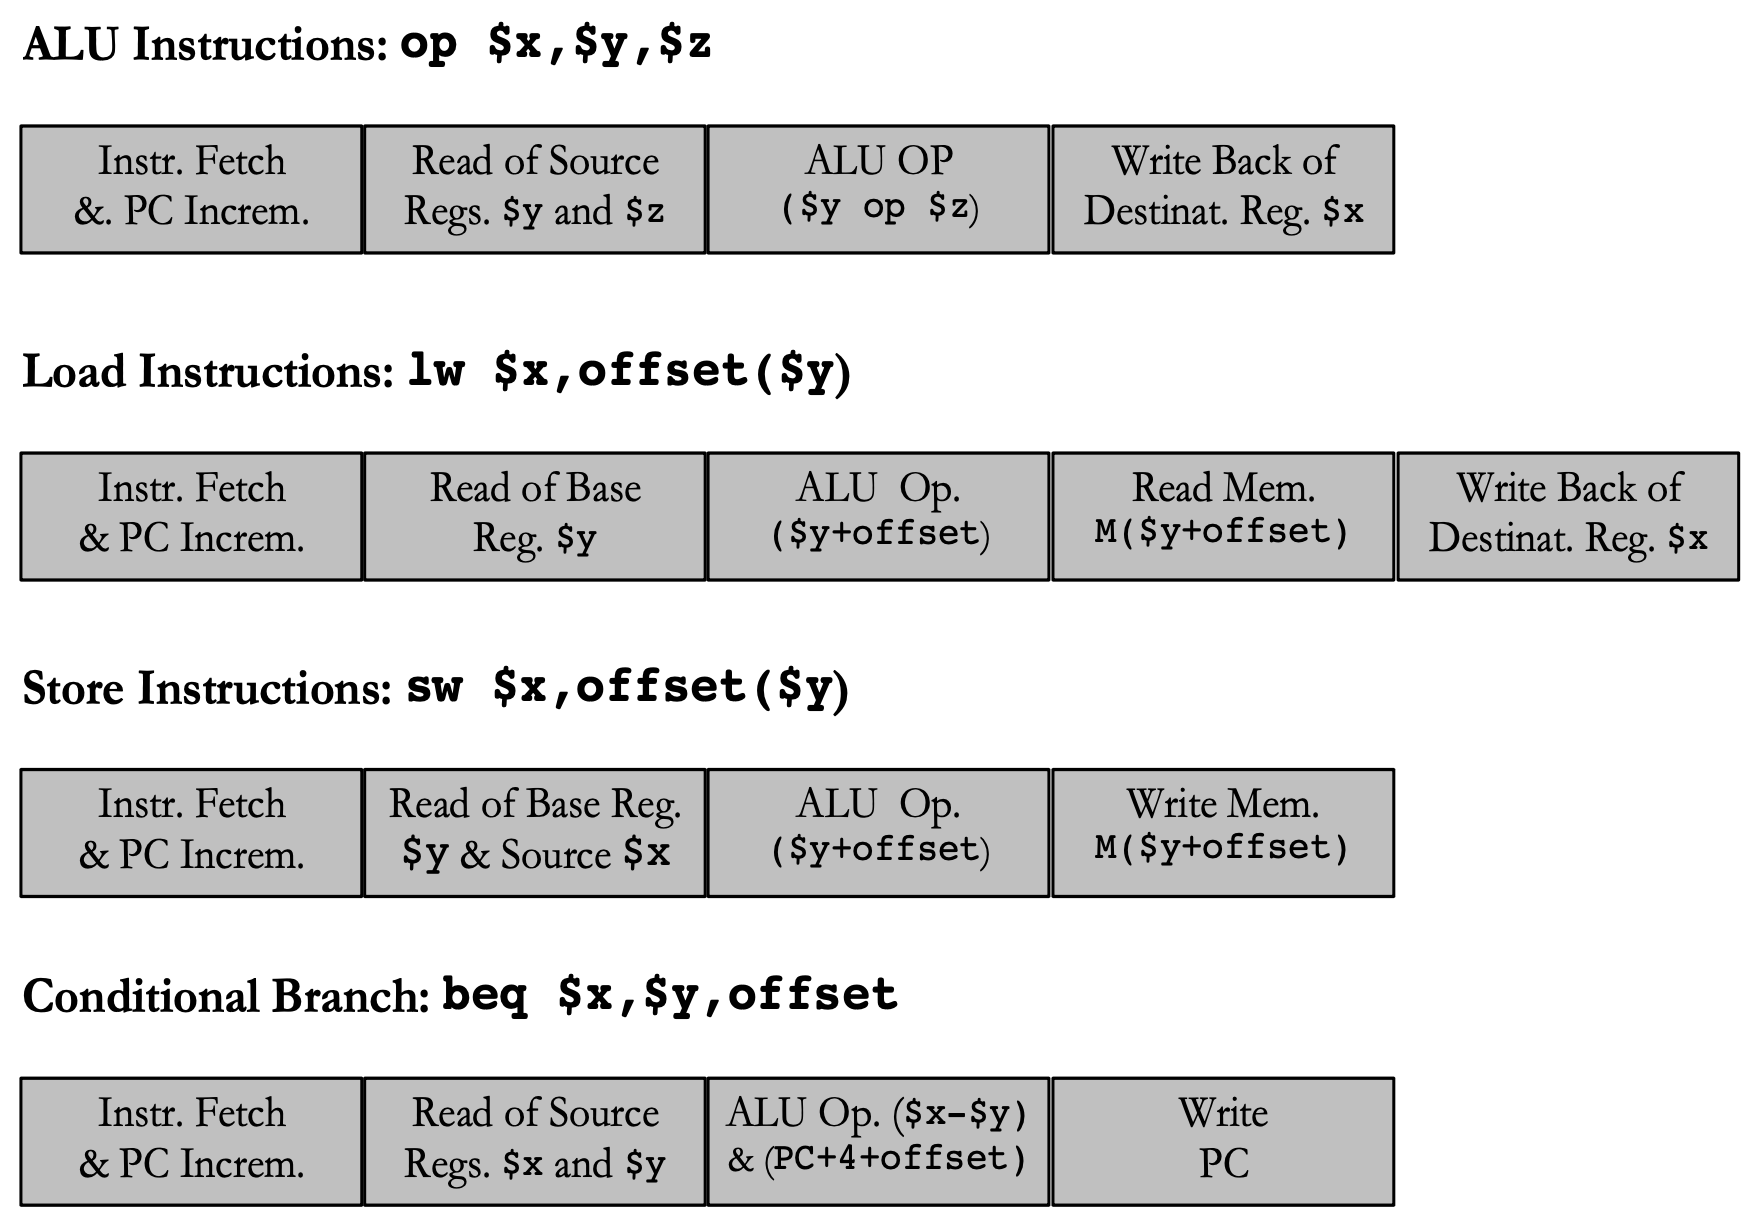
\includegraphics[scale=0.3]{images/MIPS-instructions}
    \caption{MIPS instructions}
    \label{fig: MIPS instructions}
\end{figure}

The CPU, central process unit, amounts to a control unit plus a data path.
Communication between the CPU and the memory in the computing infrastructure happens through the control, data and
address buses.

\begin{figure}[h]
    \centering
    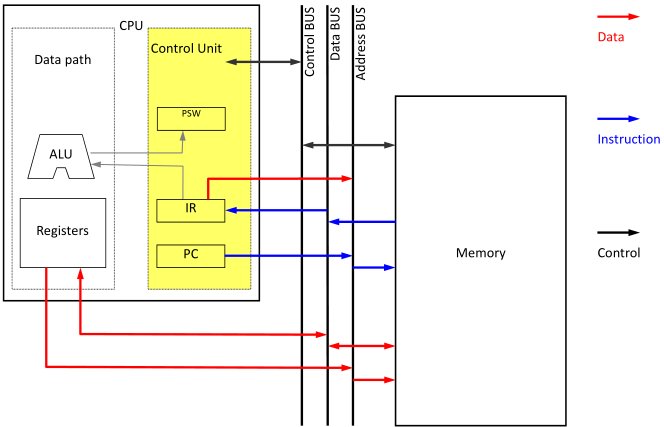
\includegraphics[scale = 0.3]{images/computing-infrastructure}
    \caption{Computing infrastructure}
    \label{fig:computing-infrastructure}
\end{figure}

\paragraph{Execution of MIPS instructions} Every instruction in MIPS subset can be implemented in at most 5 clock
cycles as follows:
\begin{description}
    \item[IF] Instruction Fetch Cycle\\
        Send the content of Program Counter register to Instruction Memory and fetch the
        current instruction from Instruction Memory.

        Update the PC to the next sequential address by adding 4 to the PC (since each instruction is 4 bytes).

    \item[ID] Instruction Decode and Register Read Cycle\\
        Decode the current instruction (fixed-field decoding)
        and read from the Register File of one or two registers
        corresponding to the registers specified in the
        instruction fields.

        Sign-extension of the offset field of the instruction in
        case it is needed.

    \item[EX] Execution Cycle\\
    The ALU operates on the operands prepared in the
    previous cycle depending on the instruction type:
    \begin{itemize}
        \item[-] Register-Register ALU Instructions: ALU executes the specified operation on the operands read
        from the RF
        \item[-] Register-Immediate ALU Instructions:
        ALU executes the specified operation on the first operand
        read from the RF and the sign-extended immediate operand
        \item[-] Memory Reference:
        ALU adds the base register and the offset to calculate the
        effective address.
        \item[-] Conditional branches:
        Compare the two registers read from RF and compute the
        possible branch target address by adding the sign-
        extended offset to the incremented PC\@.
    \end{itemize}


    \item[ME] Memory Access\\
        Load instructions require a read access to the Data
        Memory using the effective address.

        Store instructions require a write access to the Data
        Memory using the effective address to write the data
        from the source register read from the RF\@.

        Conditional branches can update the content of the PC
        with the branch target address, if the conditional test
        yielded true.

    \item[WB] Write-Back Cycle\\
        Load instructions write the data read from memory in
        the destination register of the RF\@.

        ALU instructions write the ALU results into the
        destination register of the RF\@.
\end{description}


\begin{figure}[h]
    \centering
    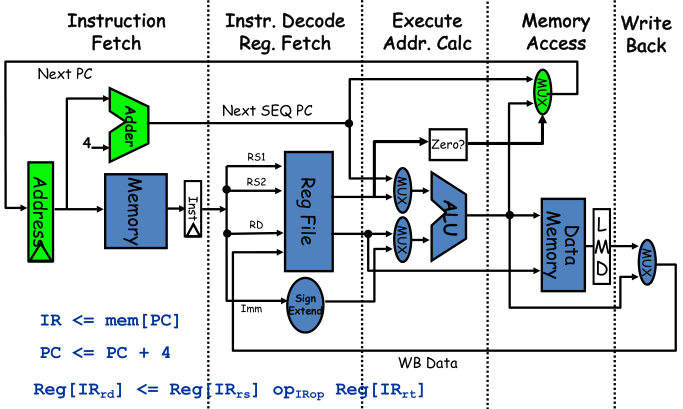
\includegraphics[scale = 0.35]{images/MIPS-data-path}
    \caption{MIPS data path}
    \label{fig:mips-data-path}
\end{figure}

In the single cycle implementation of MIPS the length of the clock cycle is defined by the critical path given by the
load instruction: T = 8ns.
Each instruction is executed in a single clock cycle of 8ns.
\begin{figure}[h]
    \centering
    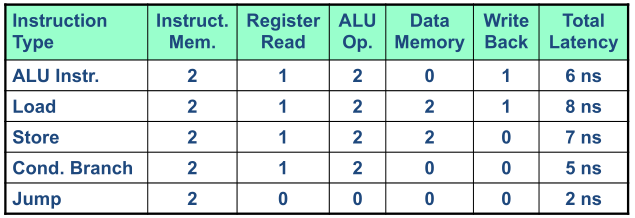
\includegraphics[scale=0.38]{images/instructions-latency}
    \caption{Instruction latency}
    \label{fig:instruction-latency}
\end{figure}

In the multi-cycle implementation the instruction is distributed on multiples cycle (5 for MIPS).

The basic cycle is smaller of 2 ns, the instruction latency is 10 ns.

The multi-cycle execution can be sequential of pipelined.
\begin{figure}[h]
    \centering
    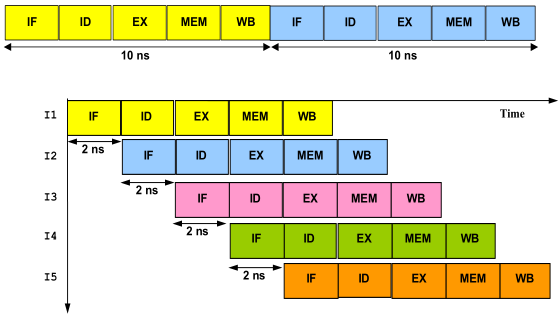
\includegraphics[scale=0.4]{images/sequential-vs-pipelined}
    \caption{Sequential vs pipelined execution}
    \label{fig:sequential-vs-sequential}
\end{figure}

\paragraph{Latency} Each instruction is worsened from 8ns to 10ns.\\
\textbf{Throughput} Is improved by four times, 1 instruction each 8ns to 1 instruction each 2ns.


The Register File is used in WB and ID stages.
In the \textbf{optimized pipeline} the RF-write in the first half of the clock cycle and the RF-read occurs in the
second half of the clock cycle avoiding a possible read after write hazard which otherwise would've required a stall.
It is safely to assume that the optimized pipeline will be the standard pipeline throughout the course.
    %! Author = lazza
%! Date = 02/05/2022

\section{Hazards}\label{sec:hazards}
Dependencies are created at code-level and can be translated into conflicts when the compiler translate the code into
instructions.

A hazard is created whenever there is a conflict (and therefore a dependency) between instructions, and
these instructions are close enough that the overlap caused by pipelining would change the order of access to the
operands involved in the dependence.

Hazards prevent the next instruction in the pipeline from executing during its designated clock cycle, reducing the
performance from the ideal speedup gained by pipelining.

\subsection{Structural hazards}\label{subsec:structural-hazards}
Use of the same resource, such as the ALU, from different instructions simultaneously.
There cannot be structural hazards in the MIPS architecture:
\begin{description}
    \item[] Instruction Memory separated from Data Memory, thus allowing the fetch of instructions and the reading of
    register during the same clock cycle.
    \item[] Register File (RF) can be accessed twice in the same clock cycle: write access on the rising edge of
    the clock and read access on the falling edge by another instruction.
\end{description}

\subsection{Data Hazard}\label{subsec:data-hazard}
Attempt to use a result before it is ready, three different types:
\begin{itemize}
    \item[] RAW, read after write
    \item[] WAR, write after read
    \item[] WAW, write after write
\end{itemize}

\begin{figure}[h]
    \centering
    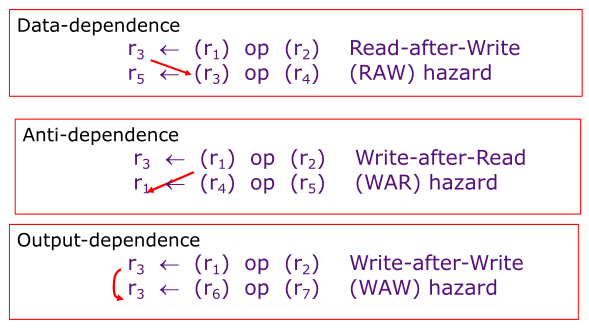
\includegraphics[scale = 0.4]{images/data-hazards-1}
    \caption{Data hazards}
    \label{fig:data-hazards}
\end{figure}


The RAW hazard is the only possible hazard in the MIPS architecture since all five stages are accessed in the
same order in and between instructions, this is due to the fact that in the MIPS architecture there cannot
be simultaneous access to the same resource and the access to the resources follow the order of the instructions.

For this reason write backs are in-order and therefore WAW cannot happen, and the reading of registers of a previous
instruction happens always before the write back of a subsequent instruction precluding the WAR hazards.

RAW hazards can be dealt with at compile-time (design solution) or at run-time (hardware solution).

\paragraph{Compilation Techniques}
\begin{itemize}
    \item[\textrightarrow] Nop instructions, insertion of no operation
    \item[\textrightarrow] Instruction Scheduling, to avoid that correlating instructions are too close the compiler
    tries to insert independent instructions among correlated instructions.
\end{itemize}
Scheduling is a reordering of independent instructions without changing the overall result;
when the compiler does not find independent instructions, it inserts nops.

\paragraph{Hardware Techniques}
\begin{itemize}
    \item[\textrightarrow] Insertion of stalls (or bubbles) in the pipeline
    \item[\textrightarrow] Data Forwarding (or Bypassing)
\end{itemize}

Forwarding data means shortcutting data from one resource of the CPU as output to another resource of the CPU as
input using one clock cycle for the propagation, this means using temporary result stored in the pipeline instead of
waiting for the write back of results in the RF\@.
Forwarding costs are additional multiplexers to allow to fetch inputs from the pipeline.\\
In the MIPS architecture the common paths for data forwarding are EX-EX, MEM-EX, MEM-MEM\@.

Note that WB-ID is not a data path, data is written and accessed in the same clock cycle inside the Register File.
MEM-ID path is not useful if we divide clock cycle in rising and falling edge (optimized pipeline).


\begin{figure}[h]
    \centering
    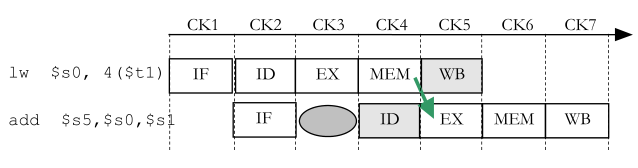
\includegraphics[scale=0.4]{images/load-use-hazard}
    \caption{Load/Use hazard requires a stall to use the MEM-EX path}
    \label{fig:load-use-hazard}
\end{figure}


\begin{figure}[h]
    \centering
    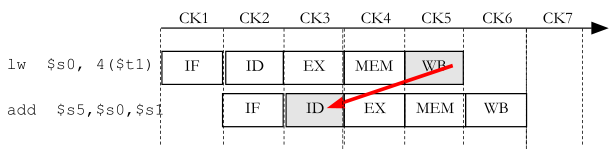
\includegraphics[scale=0.4]{images/load-use-without-forwarding}
    \caption{Load/Use without forwarding needs two stalls}
    \label{fig:load-use-without-forwarding}
\end{figure}


\begin{figure}[h]
    \centering
    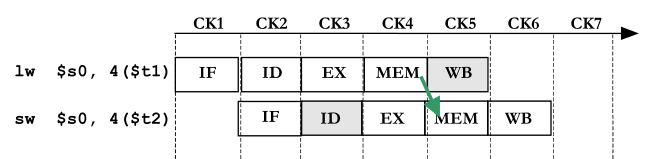
\includegraphics[scale=0.4]{images/load-store-hazard}
    \caption{Load/Store hazard uses the MEM-MEM path}
    \label{fig:load-store-hazard}
\end{figure}


\subsection{Control hazards}\label{subsec:control-hazards}
Attempt to make a decision on the next instruction to execute, before the condition is evaluated.
A MUX is responsible for the value of PC, which is based on ALU output: until the ALU doesn't evaluate the
condition the PC is not known, and we can't know which is the next instruction.

The PC is available at the MEM stage.

Generally true statements are executed in the waiting for the evaluation, as if the condition
were true and no jump was needed: just add to the PC plus one, and then see if the branch is taken.
For this particular reason it is suggested to write inside the \verb|IF| statements the code that most probably is
going to be executed.

In case we wait for the evaluation of the condition the stalls required are two in case of forwarding, three without forwarding.
%add figure explaing

An additional solution would be the early evaluation of the PC in the ID stage instead of the EXE stage, in this new
pipeline the PC adder is anticipated and only one stall would be required (with forwarding) to fetch the correct instruction.
This solution bring an issue in presence of a RAW hazard: anticipating the PC adder means that we have to add a stall
in order to solve the conflict.

\begin{figure}[h]
    \centering
    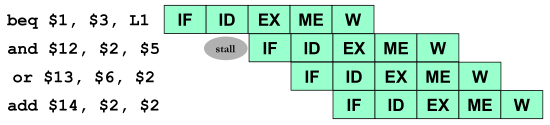
\includegraphics[scale = 0.4]{images/pc-early-evaluation}
    \caption{Early evaluation of the PC}
    \label{fig:pc-early-evaluation}
\end{figure}

\begin{figure}[h]
    \centering
    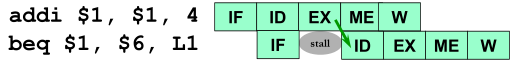
\includegraphics[scale = 0.4]{images/pc-early-evalutation-issue}
    \caption{PC early evaluation issue}
    \label{fig:pc-early-evaluation-issue}
\end{figure}
    %! Author = lazza
%! Date = 02/05/2022

\section{Branch prediction}\label{sec:branch-prediction}
When a branch is taken the \textbf{branch target address} (BTA) is stored in the PC instead of the address of the
next instruction in the sequential instruction stream.
The branch outcome and Branch Target Address are ready at the end of the EX stage, conditional branches are solved
when PC is updated at the end of the ME stage.
Control hazards reduce the performance from the ideal speedup gained by the pipelining since they can
make it necessary to stall the pipeline.

\begin{figure}[h]
    \centering
    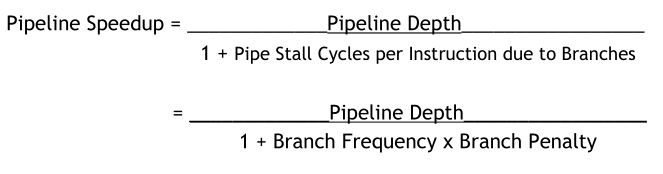
\includegraphics[scale = 0.35]{images/performace-impact-control-hazards}
    \caption{Performance impact by control hazards}
    \label{fig:performance-impact-by-control-hazards}
\end{figure}


\begin{figure}[h]
    \centering
    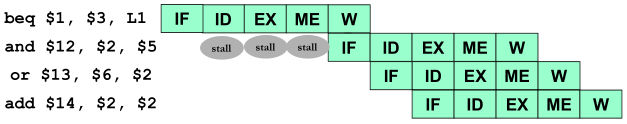
\includegraphics[scale = 0.4]{images/branch-without-forwarding}
    \caption{Branch stalls without forwarding}
    \label{fig:branch-stalls-without-forwarding}
\end{figure}

\begin{figure}[h]
    \centering
    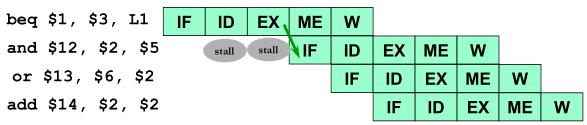
\includegraphics[scale = 0.4]{images/branch-with-forwarding}
    \caption{Branch stalls with forwarding}
    \label{fig:branch-stalls-with-forwarding}
\end{figure}

In order to reduce the speed penalty cause by the branch hazards we can use prediction techniques in order to guess
the next instruction to be executed.

\subsection{Static branch prediction}\label{subsec:static-branch-prediction}
Static branch prediction are at compile-time:
\begin{itemize}
    \item Branch always taken - No jump
    \item Branch always not taken\\ In theory always jump, but in reality we have to calculate the BTA before jumping
    and at this point there is no prediction to make (at least in the MIPS pipeline).
    \item Backward taken, forward not taken\\
    Based on the assumption that backward jumps (while and for loops) are taken and forward jumps (if statements) are
    not taken.
    \item Profile driven prediction\\
    We are going make several runs of our program and the choice is based on statistical data for each branch.
    \item Delayed Branch\\
    The compiler statically schedules and independent instruction in the branch delay slot, which is executed whether
    the branch is taken.
    %The independent instruction can belong also to the branch.
    There are three ways in which the branch delay slot can be scheduled:
        \subitem From before, the instruction in the delay slot is always executed.
        \subitem From target, this strategy is preferred when the branch is taken with high probability.
        \subitem From fall-through, this strategy is preferred when the branch is not taken with high probability. In
    this case the branch delay slot is scheduled from the not-taken fall-through path.
\end{itemize}

\begin{figure}[h]
    \centering
    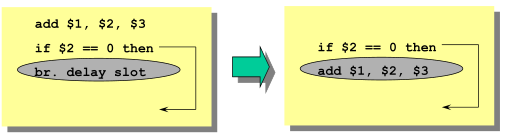
\includegraphics[scale = 0.4]{images/branch-delayed-from-before}
    \caption{Branch delayed - from before}
    \label{fig:branch-delayed-from-before}
\end{figure}

\begin{figure}[h]
    \centering
    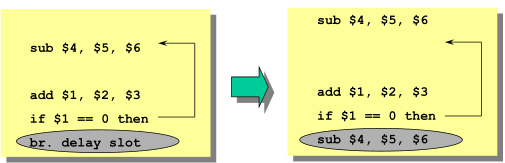
\includegraphics[scale = 0.4]{images/branch-delayed-from-target}
    \caption{Branch delayed - from target}
    \label{fig:branch-delayed-from-target}
\end{figure}

\begin{figure}[h]
    \centering
    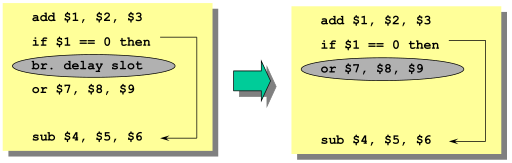
\includegraphics[scale = 0.4]{images/branch-delayed-from-fall-through}
    \caption{Branch delayed - from fall-through}
    \label{fig:branch-delayed-from-fall-through}
\end{figure}


\subsection{Dynamic branch prediction}\label{subsec:dynamic-branch-prediction}
Dynamic branch prediction happens at run-time by the hardware, and is based on two interacting mechaninsms:
\begin{itemize}
    \item Branch Outcome Predictor\\
    To predict the direction of a branch (i.e., taken or not taken).
    \subitem Branch History Table
    \item Branch Target Predictor\\
    To predict the branch target address in case of taken branch.
    \subitem Branch Target Buffer
\end{itemize}

\subsubsection{Branch Target Buffer}
The Branch Target Buffer (BTB or Branch Target Predictor) is a cache storing the predicted branch target address
for the next instruction after a branch.
We access the BTB in the IF stage using the instruction address of the fetched instruction (a possible branch) to
index the cache.

\begin{figure}[H]
    \centering
    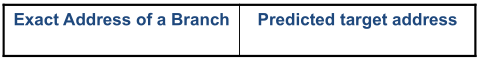
\includegraphics[scale = 0.4]{images/branch-target-buffer-entry}
    \caption{BTB entry}
    \label{fig:btb-entry}
\end{figure}

%In reality we cannot index all the possible branches since the BTB has a fixed size, the entry will not contain the
%exact address of a branch but only the last n-bits of the address, allowing the possibility for collisions.

\subsubsection{Branch History Table}
The Branch History Table (BHT or Branch Prediction Buffer) is indexed by the last k-bits of the branch address, meaning
that there are at most $2^k$ entries, with possible collisions, and each entry contains n-bits that says whether the
branch was recently taken.

\begin{figure}[H]
    \centering
    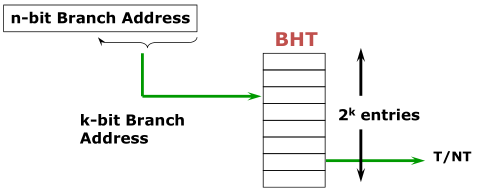
\includegraphics[scale = 0.4]{images/branch-history-table}
    \caption{Branch history table}
    \label{fig:branch-history-table}
\end{figure}

The 1-bit history table tells us if the last time the branch was taken or not taken (e.g., 0 and 1).
Differently from the profile drive prediction the BHT is updated whenever the branch is encountered.

For example:\\
0, prediction not taken, outcome not taken - no update\\
0, prediction not taken, outcome taken - update 0 to 1\\
0, prediction taken, outcome not taken - update 1 to 0\\

\begin{figure}[h]
    \centering
    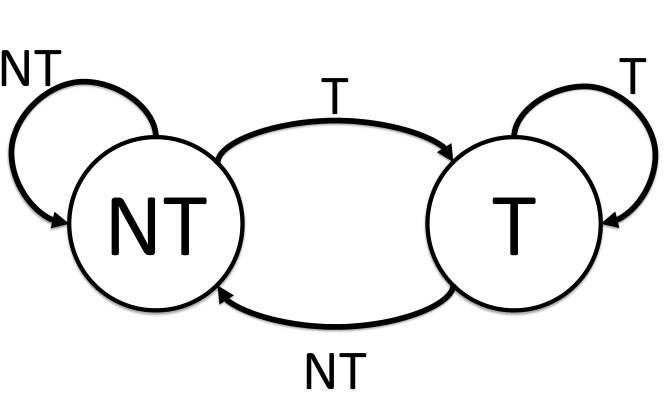
\includegraphics[scale = 0.15]{images/1-bit-BHT-automata}
    \caption{1-bit BHT automata}
    \label{fig:1-bit-BHT-automata}
\end{figure}

A misprediction occurs when:
\begin{itemize}
    \item[\textrightarrow] The prediction is incorrect for that branch
    \item[\textrightarrow] The same index has been referenced by two different branches, and the previous history
    refers to the other branch.
    To solve this problem it is enough to increase the number of rows in the BHT or to use a hashing function.
\end{itemize}

Among the n-bits BHT the 2-bit history table is the best one because it is still small in size, it allows for speedy
updates maintaining
the prediction accuracy high, but differently from the 1-bit the prediction must miss twice before it is changed.
In a loop branch we do not need to change the prediction at the last iteration, thus increasing the speed in case of
nested loop such as the ones used to inspect matrices.

\begin{figure}[h]
    \centering
    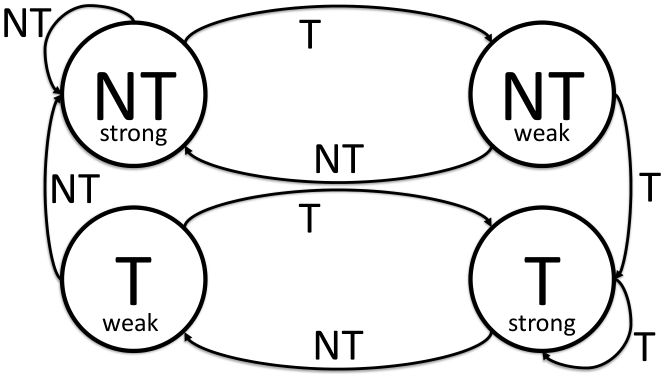
\includegraphics[scale = 0.2]{images/2-bit-BHT-automata}
    \caption{2-bit BHT automata}
    \label{fig:2-bit-BHT-automata}
\end{figure}

\begin{figure}[h]
    \centering
    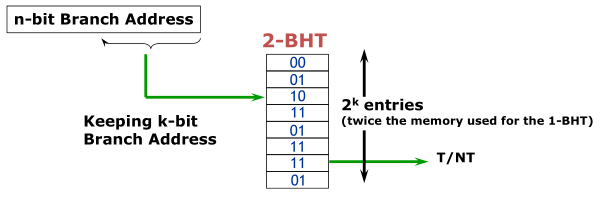
\includegraphics[scale = 0.3]{images/2-bit-BHT}
    \caption{2-bit BHT}
    \label{fig:2-bit-BHT}
\end{figure}


\subsubsection{Correlating Branch Predictor}
The idea behind is that the behaviour of recent branches are correlated, that is the recent behaviour of other
branches can influence the prediction of the current branch.
In general (m, n) correlating predictor records last m branches to choose from $2^m$ BHTs, each of which is a n-bit
predictor.
The branch prediction buffer can be indexed by
using a concatenation of low-order bits from the
branch address with m-bit global history (i.e.,
global history of the most recent m branches).

Example: a (2, 2) correlating predictor with 64 total entries;
6-bit index composed of: 2-bit global history and 4-bit low-
order branch address bits.

\begin{figure}[H]
    \centering
    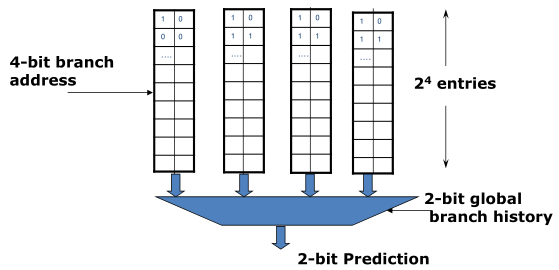
\includegraphics[scale = 0.4]{images/(2,2)-correlating-branch-predictor}
    \caption{(2,2) correlating branch predictor}
    \label{fig:(2,2)-correlating-branch-predictor}
\end{figure}

The (2,2) correlating branch predictor outperforms other predictors such as the 2-bit BHT.
    %! Author = lazza
%! Date = 03/05/2022

\section{Instruction level parallelism}\label{sec:instruction-level-parallelism}
ILP: potential overlap of execution among unrelated instructions, possible if:
\begin{itemize}
    \item no structural hazards
    \item no raw, waw, war stalls
    \item no control hazards
\end{itemize}

\begin{center}
    Pipeline CPI = Ideal pipeline CPI + Structural Stalls +\\Data Hazards Stalls + Control Stalls
\end{center}

In the MIPS architecture the only possible structural hazards, WB-ID, where a register in the RF can be both written
and read, is solved by splitting the clock cycle in rising edge (WB) and falling edge (ID).


\begin{table}[h]
    \centering
    \begin{tabular}{|p{3cm}|p{3.5cm}|}
        \toprule
        \textbf{ILP} & \textbf{PP} \\
        \midrule
        overlap individual machine operations & separate processor getting separate chuncks of the program \\
        \midrule
        transparent to the user & nontransparent to the user \\
        \midrule
        goal: speed up & goal: speed up and quality up \\
        \bottomrule
    \end{tabular}
    \caption{ILP vs Parallel Processing}
    \label{tab:ILP-vs-PP}
\end{table}


\subsection{Complex Pipeline}\label{subsec:complex-pipeline}
WAR and WAW were not possible with ADD operation with integers, but MULT and DIV operations use floating point numbers.
A new stage introduced, the ISSUE stage, that allows for high performance in presence of:
\begin{itemize}
    \item long latency or partially pipeline floating-point units
    \item multiple function and memory units
    \item memory systems with variable access time
    \item precise exception
\end{itemize}

\begin{figure}[h]
    \centering
    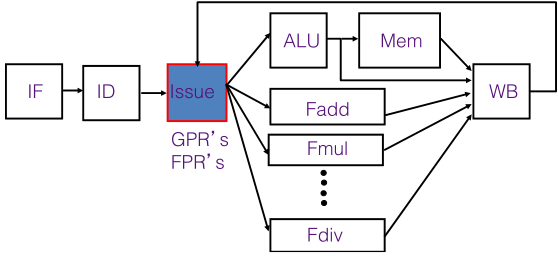
\includegraphics[scale = 0.4]{images/complex-pipeline}
    \caption{Complex pipeline}
    \label{fig:complex-pipeline}
\end{figure}

New hazards arise from variable latencies of different FUs:
\begin{itemize}
    \item Structural
    \begin{itemize}
        \item EX stage if some FPU or memory unit is not pipelined and takes more than one cycle.
        \item WB stage due to variable latencies of different functional units
    \end{itemize}
    \item Data
    \begin{itemize}
        \item WAW due to variable latencies of the FUs
    \end{itemize}
\end{itemize}

A solution would be delay the WB in order to have the same latency for all instructions but that would slow down too
much single cycle integer operations without forwarding.

\paragraph{When it is safe to issue an Instruction?} Things to consider before dispatching an instruction:
\begin{itemize}
    \item the required FU is available
    \item the input data is available
    \item it is safe to write the destination
    \item there is not a structural conflict at the WB stage
\end{itemize}

\paragraph{Assumptions} Of a general complex pipeline architecture:
\begin{itemize}
    \item all functional units are pipelined
    \item registers are read in ISSUE stage: we consider that a register is written (WB) in the first half of the clock
    cycle and read (IS) in the second half of the clock cycle
    \item no forwarding
    \item ALU operations take 1 clock cycle
    \item FP ALU operations take 2 clock cycles
    \item memory operations take 2 clock cycles
    \item write back unit has a single port
    \item instructions are fetched, decoded and issued in order
    \item an instruction will only enter the ISSUE stage if it does not cause a WAR or WAW hazard
    \item only one instruction can be issued at a time, and in the case multiple instructions are ready, the oldest
    one will go first
\end{itemize}


To reach higher performance more parallelism must be achieved, this cannot be done augmenting the CPI of the ideal
pipeline because it could create further problems with hazards.

Dependences must be detected and solved, and
instructions must be ordered (scheduled) so as to
achieve highest parallelism of execution compatible
with available resources.

Three types of dependencies:
\begin{itemize}
    \item data dependencies, RAW
    \item control dependencies
    \item name dependencies, two types:
    \begin{itemize}
        \item antidependencies, WAR
        \item output dependencies, WAW
    \end{itemize}
    Generated by the lack of registers.
\end{itemize}

Dependencies are a property of the program, while
hazards are a property of the pipeline.


The main techniques to eliminate dependencies are:
\begin{itemize}
    \item register renaming
    \item scheduling
    \begin{itemize}
        \item static, compiler
        \item dynamic, hardware
    \end{itemize}
\end{itemize}
%-> superscalar

Steps to exploit more ILP in terms of hardware optimization:
\begin{itemize}
    \item[\textrightarrow] sequential
    \begin{itemize}
        \item[$\hookrightarrow$] pipeline\\ single-issue in-order-execution
        \begin{itemize}
            \item[$\hookrightarrow$] dynamic scheduling\\ single-issue out-of-order execution
            \begin{itemize}
                \item[$\hookrightarrow$] superscalar\\ multiple-issue out-of-order execution
            \end{itemize}
        \end{itemize}
    \end{itemize}
\end{itemize}

\begin{figure}
    \centering
    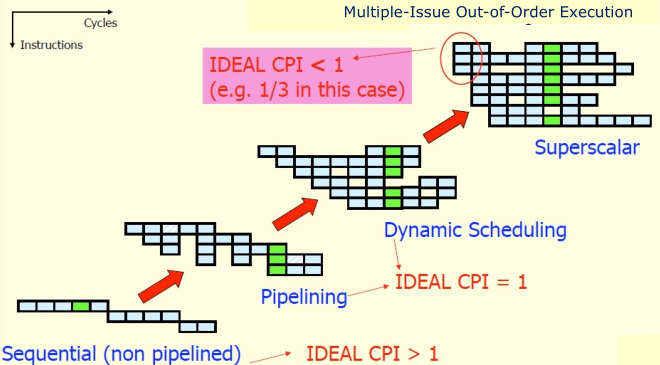
\includegraphics[scale = 0.35]{images/ILP-scheme}
    \caption{Instruction Level Parallelism}
    \label{fig:ILP-scheme}
\end{figure}

    %! Author = lazza
%! Date = 03/05/2022

\section{Static scheduling}\label{sec:static-scheduling}
Compilers can use sophisticated algorithms for code
scheduling to exploit ILP\@.
The amount of parallelism available within a \textbf{basic block}, a straight-line code sequence with no branches in
except to the entry and no branches out except at the
exit, is quite small (statistically it varies from 4 to 7 instructions).

Data dependence can further limit the amount of ILP we
can exploit within a basic block to much less than the
average basic block size.

To obtain substantial performance enhancements, we
must exploit ILP across multiple basic blocks (i.e.,
across branches).

Static detection and resolution of dependencies are accomplished by the compiler, dependencies are avoided by code
reordering.

The output of the compiler is a reordered dependency-free code, which can be processed, for example, by the VLIW (Very
Long Instruction Word) processors.

\paragraph{Limits of Static Scheduling}
\begin{itemize}
    \item unpredictable branches
    \item variable memory latency
    \item code size explosion
    \item compiler complexity
\end{itemize}

Till know we had a single-core multi-cycle parallelism, thanks to the single-issue pipelined architecture.
The single-issue architecture means we cannot aim to have an ideal CPI bigger than one.

Multi-issue architectures are the next step to improve the CPI:
\begin{itemize}
    \item Superscalar
    \item VLIW
\end{itemize}

\subsection{VLIW architectures}\label{subsec:vliw-architectures}
Each instruction word contains more than one operation, the processor can initiate multiple operations per cycle
specified completely by the compiler.
This leads to a low hardware complexity:
\begin{itemize}
    \item no scheduling
    \item reduced support of variable latency instructions
    \item single control flow (1 PC)
    \item explicit parallelism
\end{itemize}

An instruction can be a set of operations that are intended to be issued simultaneously, the VLIW has multiple
operations packed into one instruction, and each type of operation has its own slot.

\begin{figure}[h]
    \centering
    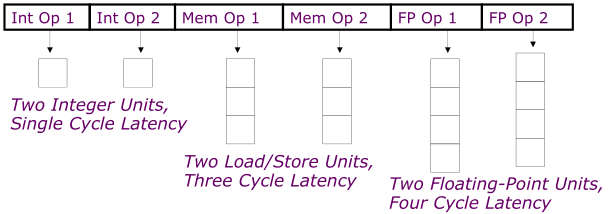
\includegraphics[scale = 0.4]{images/vliw}
    \caption{Very Long Instruction Word}
    \label{fig:vliw}
\end{figure}

This type of architecture requires guarantees of:
\begin{itemize}
    \item parallelism within an instruction does not generate RAW data hazard
    \item no data use before the data is ready, no data interlocks
\end{itemize}

Compiler responsibilities:
\begin{itemize}
    \item maximize parallel execution
    \begin{itemize}
        \item exploit ILP and LLP (Loop Level Parallelism)
        \item it is necessary to map the instructions over the machine functional units
        \item this mapping must account for time constraints and dependencies among the tasks
    \end{itemize}
    \item guarantee intra instruction parallelism
    \item avoid hazards (no interlocks), typically separates operations with explicit nops
    \item minimize the total execution time
\end{itemize}


\paragraph{Pros:}
\begin{itemize}
    \item[] simple HW
    \item[] good compilers can effectively detect parallelism
\end{itemize}
\paragraph{Cons:}
\begin{itemize}
    \item huge number of registers to keep active the FUs
    \begin{itemize}
        \item needed to store operands and results
    \end{itemize}
    \item large data transport capacity between
    \begin{itemize}
        \item FUs and register files
        \item Register files and Memory
    \end{itemize}
    \item high bandwidth between i-cache and fetch unit
    \item large code size
    \begin{itemize}
        \item use of (big) nops in the VLIW
        \item unpredictable branches have different optimal schedules that varies with branch path
    \end{itemize}
    \item knowing branch probabilities requires significant extra steps in build process due to profiling
\end{itemize}


An example of scheduling of a loop in VLIM architecture:
\begin{table}[h]
    \centering
    \begin{tabular}{c|c|c|c}
        \toprule
        operations & \textbf{ls, sd} & \textbf{add, bne} & \textbf{fadd} \\
        \midrule
        clock cycles & 3 & 1 & 4\\
        \bottomrule
    \end{tabular}
    \label{tab:}
\end{table}

\begin{figure}[h]
    \centering
    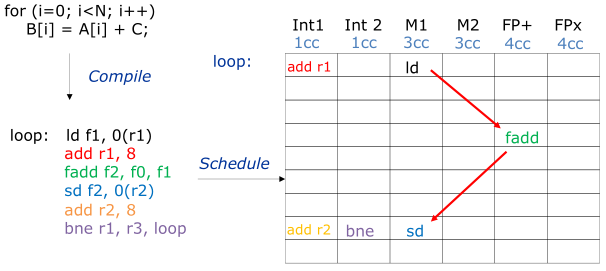
\includegraphics[scale = 0.4]{images/vliw-no-loop-unrolling}
    \caption{Loop execution on VLIM}
    \label{fig:vliw-no-loop-unrolling}
\end{figure}

Many blank lines in the scheduler corresponds to nops, leading to \(\frac{1\text{ FP ops}}{8\text{ cycles}} = 0,125\)
, which is far from our ideal CPI > 1.
To increase parallelism we use loop unrolling.

\clearpage
\subsection{Loop unrolling}
The idea is that we can extend the loop body as to include a finite number of subsequent iterations of the loop,
increasing the amount of available ILP\@.
Unrolling simply replicates the loop body multiple times, adjusting the loop termination code, by doing so the loop
\textit{overhead} decrease relatively to the loop \textit{body}.

\begin{center}
    Loop = (loop prolog + \(4\, \times\)\textit{loop body} + loop epilog) \texttimes $\, \frac{n}{4}$ iterations
\end{center}

\begin{figure}[h]
    \centering
    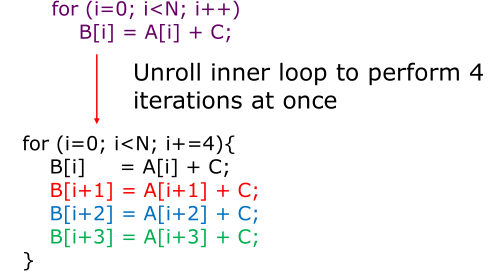
\includegraphics[scale = 0.4]{images/loop-unrolling-1}
    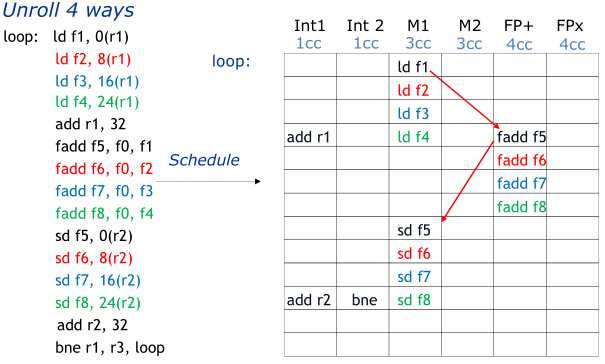
\includegraphics[scale = 0.4]{images/loop-unrolling-2}
    \caption{Loop unrolling}
    \label{fig:loop-unrolling}
\end{figure}

Note that non FP operations can have multiple schedule locations, e.g., the \verb|ld f2| could be scheduled also in
the first cycle to M2, but if does not decrease the CPI, it is recommended using a new instruction.
In this case we end up with \(\frac{4\text{ FP ops}}{11\text{ cycles}} \approx 0,36\), more than doubling the
previous result.

The \textbf{limits} of loop unrolling:
\begin{itemize}
    \item[] code size
    \item[] number of register
\end{itemize}
That is, we have an upper bound to the number of replications of the loop body, which has to be considered constant
in regard to the $\theta(n)$ loop iterations: we reduced the \textit{prolog} and \textit{epilog} of the loop by
a constant.

We can optimize the results of loop unrolling with \textbf{software pipelining}, further increasing the ILP\@.
\begin{figure}[h]
    \centering
    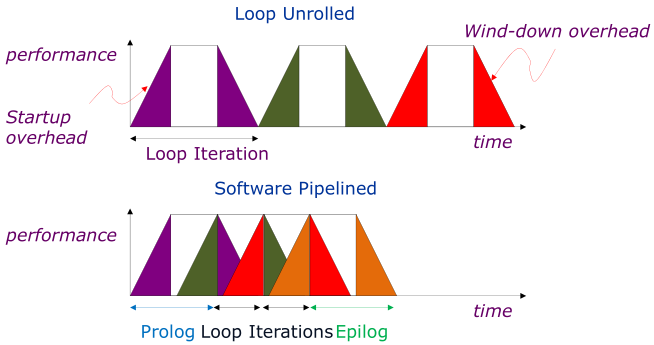
\includegraphics[scale = 0.4]{images/loop-unrolled-vs-software-pipelined-1}
    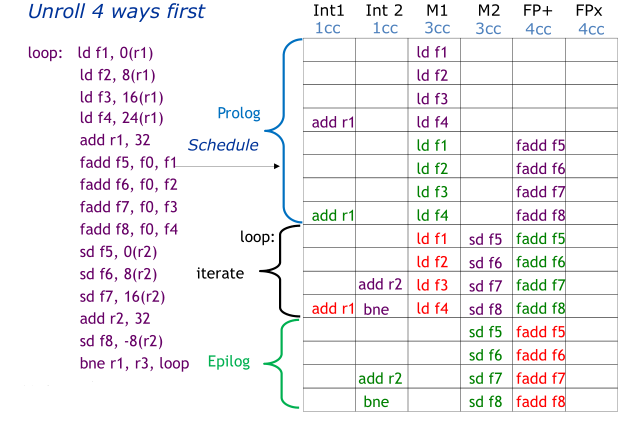
\includegraphics[scale = 0.4]{images/loop-unrolled-vs-software-pipelined-2}
    \caption{Loop unrolled vs Software pipelined}
    \label{fig:loop-unrolled-vs-sw-pipelined}
\end{figure}

\begin{center}
    Software Pipelined Loop = prolog + \textit{iterations} + epilog
\end{center}

In this case we have just one prolog and one epilog for all the loop iterations and can be considered $O(1)$ with
respect to the $n$ iterations.
For this reason we consider only the \textit{iterate} part for our performance evaluation which is \(\frac{4\text{ FP
ops}}{4\text{ cycles}} = 1\).

\textbf{Note:} in case of short loops, loop unrolling looses performance due to the costs of starting and closing the
iterations.

\clearpage
\subsection{Trace Scheduler}\label{subsec:trace-scheduler}
Loop unrolling is useful but does not cover other type of branches that limit the basic \textbf{block size} in
control-flow intensive irregular code.
In these cases is difficult to find ILP in individual basic blocks.

Trace scheduling focus on traces:
\begin{itemize}
    \item a loop-free sequence of basic blocks embedded in the control flow graph
    \item it is an execution path which can be taken for some set of inputs
    \item the chances that a trace is actually executed depends on the input set that allows its execution
\end{itemize}

\textbf{Note:} a trace may include branches but not loops.

\paragraph{Algorithm} Idea, some traces are executed much more frequently than others:
\begin{itemize}
    \item pick string of basic blocks, a trace, that represents most frequent branch path
    \item use profiling feedback or compiler heuristics to find common branch paths
    \item schedule whole "trace" at one
    \item add fixup code to cope with branches jumping out of trace
\end{itemize}
\begin{figure}[h]
    \centering
    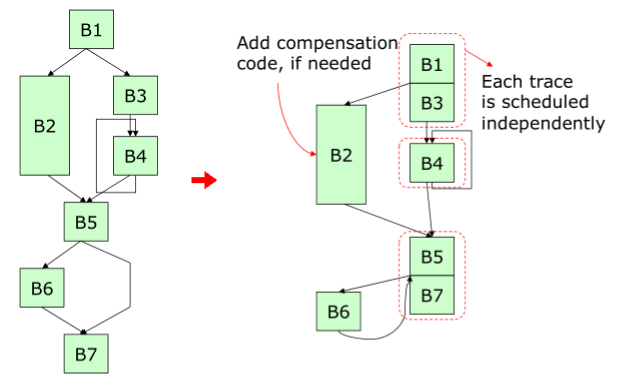
\includegraphics[scale = 0.45]{images/trace-scheduling}
    \caption{Trace scheduling}
    \label{fig:trace-scheduling}
\end{figure}

For example we suppose that \{B1, B3, B4, B5, B7\} is the most frequently executed path, therefore the traces are
\{B1, B3\}, \{B4\} and \{B5, B7\}.\\
\textbf{Note:} Traces are scheduled as if they were basic blocks, by removing control hazards we increase ILP\@.

\paragraph{Problems} Compensation codes are difficult to generate, especially entry points (of a different path).
In addition to need of compensation codes there are
restrictions on movement of a code in a trace:
\begin{itemize}
    \item \textbf{dataflow} of the program must not change, it is guaranteed to be correct by maintaining:
    \begin{itemize}
        \item data dependencies
        \item control dependencies
    \end{itemize}
    \item the exception behaviour must be preserved
\end{itemize}


\paragraph{Solutions}There are two approaches to eliminate control dependency:
\begin{itemize}
    \item use of \textbf{predicate} instructions (Hyperblock scheduling)
    \item use of \textbf{speculative} instructions (Speculative Scheduling), and speculatively move an instruction
    before the branch.
\end{itemize}

\begin{figure}[h]
    \centering
    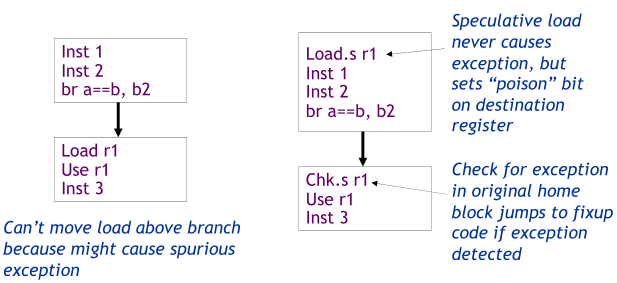
\includegraphics[scale = 0.4]{images/speculative-instruction}
    \caption{Speculative instruction}
    \label{fig:speculative-instruction}
\end{figure}

\begin{figure}[h]
    \centering
    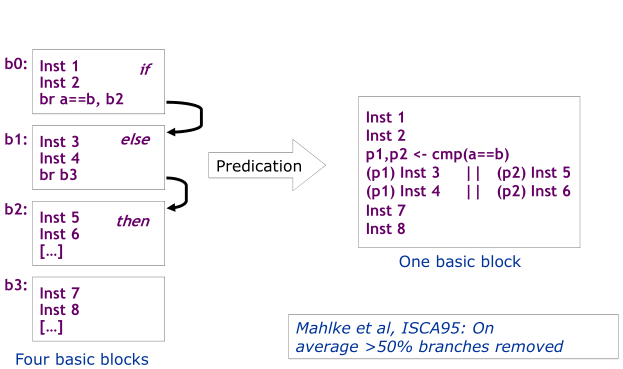
\includegraphics[scale = 0.4]{images/predicated-execution}
    \caption{Predicated execution}
    \label{fig:predicated-execution}
\end{figure}

Rotating Register Files


\clearpage
\subsection{Dynamic scheduling}\label{subsec:dynamic-scheduling}

The hardware reorders the instruction execution to reduce pipeline
stalls while maintaining data flow and exception behavior.
•
Main advantages:
– It enables handling some cases where dependences are
unknown at compile time
– It simplifies the compiler complexity
– It allows compiled code to run efficiently on a different pipeline.
•
Those advantages are gained at a cost:
– A significant increase in hardware complexity,
– Increased power consumption
– Could generate imprecise exception

Basically: Instructions are fetched and issued in program order (in-
order-issue)
•
Execution begins as soon as operands are available
– possibly, out of order execution – note: possible even with
pipelined scalar architectures.
•
Out-of order execution introduces possibility of WAR, WAW data
hazards.
•
Out-of order execution implies out of order completion unless there
is a re-order buffer to get in-order completion


    %! Author = lazza
%! Date = 03/05/2022

\subsection{Dynamic Scheduling}\label{subsec:dynamic-scheduling}

Scoreboard algo for dynamic scheduling

when is it safe to Issue an instruction slide 13
-
-
-
-

scoreboard manages commits to registers

RAW detected in ID stage, ID stage divided in two:
- instruction decode
- read registers

Scoreboard:
RAW ID stalls
WAR WB stalls
WAW not issued (stall the issue) - register renaming not used

techniques:
- register renaming

Scoreboard control structure:
1. instruction status, tells witch istr is being executed
2. functinal status, state of the functional unit
3. register result status, indicated which functional unit will write each register.

Qj and Qk tells who is going to provide the data in terms of functional unit (if not available yet)
Rj and Rk tells if the data is ready or not, prevents WAR

ADDD, DIVD, MULTD what D stands for?

in-order issue
out-of-order read
out-of-order write

-----

Tomasulo algo

load and store treated as integer FU

Common Data Bus - serialized access to write back
CDB provides values before they are saved into registers (somewhat similar to path forwarding)

FP floating point?

Reservation Station RS components
-
-
-
\ldots

STAGES
- issue
-
-

V value
Q pointer

LD: 1 cc to integer operation (offset + base address) and 1 cc to access the memory = 2 cc for Execution Completion + 1 cc to commit in the CDB

R(F4) = F4 value, register f4 Renamed

in-order issue
out-of-order execution
out-of-order write

try to do exercise on the slides

in case of concurrent writes choose the one that belongs to the critical path.

Scoreboard vs Tomasulo:
- structural hazards in scoreboard
- lack of forwarding in scoreboard


    %! Author = lazza
%! Date = 03/05/2022


Exception handling

definitions
exception :
interrupt : external of internal event that needs to be processed by another program (the interrupt handler), at the end resume normal execution

External async events:
- input output device-request
- timer expiration
- power disruptions, hardware failure

Internal sync event:
- undefined opcode, privileged instruction
- arithmetic overflow, FPU exeception
- misaligned memory access
- virtual memory exceptions: page faults, TLB misse, protection violations
- traps: system calls, e.g., jumps into kernel

Exception classes:
- synchronous vs asynchronous, asynch caused by devices external to the CPU and memory and can be handled easily
- user requested vs coerced, user requested are predictable: treated as exceptions because they use the same mechanism that are used
to save and restore the state;
handled after the instruction has completed.
Coerced are caused by some HW event not under control of the program.
- user maskable vs user nonmaskable
- within vs between instructions
- resume vs terminate

For the exam study difference between pairs.

Invoking the interrupt handler:
- terminate exec of instr till PC-4
- store the PC in EPC register, exception program counter
- disable other interrupts and transfers control to a designated interrupt running in the kernel mode

In the cpu we have two modes: user-mode and kernel-mode (unstoppable).

precise interrupts
- easy handled

Exception handling in the 5-stage pipeline

    %! Author = lazza
%! Date = 06/05/2022

\section{HW speculation}\label{sec:hw-speculation}
HW-based speculation combines three ideas:
\begin{description}[noitemsep]
    \item[Dynamic Branch Prediction] to choose which instruction to execute
    \item[Dynamic Scheduling] supporting out-of-order execution but in-order commit to prevent any irrevocable
    actions (such as register update or taking exception) until an instruction commits
    \item[Speculation] To execute instructions before control dependencies are solved
\end{description}
The idea is allowing instruction to execute freely and out-of-order, based on speculation, but allow to update the RF
or the memory only when an instruction is no longer speculative.

Mechanisms are necessary to handle incorrect speculation, hardware speculation extends dynamic scheduling beyond a
branch, i.e., behind the basic blocks.

\subsection{Reorder buffer}\label{subsec:reorder-buffer}
A buffer that holds instruction results before they are committed.
When an instruction complete execution, the results are placed into ROB, which holds the instructions in FIFO order,
exactly as issued.
The result in the ROB buffer are tagged, they are used instead of the reservation stations, supplying operands to
other instruction between execution and commit.
The instruction at the \textbf{head} of ROB can safely commit, all its predecessor have already committed.

\begin{figure}[h]
    \centering
    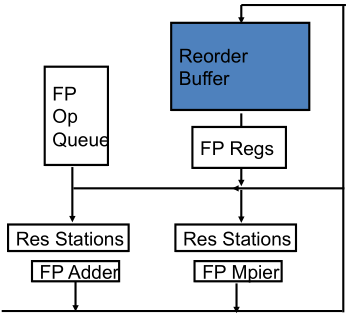
\includegraphics[scale = 0.4]{images/reorder-buffer}
    \caption{ROB}
    \label{fig:rob}
\end{figure}

\paragraph{Separating Completion from Commit} Re-order buffer holds the register result from completion until commit:
\begin{itemize}[noitemsep]
    \item[-] entries are allocated in program order during decode
    \item[-] it buffers completed values and exception state until commit point
    \item[-] completed values can be used by dependents before committed (bypassing)
    \item[-] each entry holds a program counter, instruction type, destination register specifier and value if any,
    and exception status
\end{itemize}

\paragraph{Memory reordering} It needs special data structures:
speculative store address and data buffers, speculative load address and data buffers.

\paragraph{Precise interrupts and Speculation} If a speculation is wrong, we need to be able to back and restart
execution to a point before out incorrect prediction (e.g., branch prediction), it happens the same as precise
exceptions.
The recovery technique for both is \textbf{in-order commit}.


\subsection{Speculative Tomasulo}\label{subsec:speculative-tomasulo}
\subsubsection{Stages}
\begin{description}
    \item[Issue] get instruction from FP Op Queue.\\
    If the reservation station \textcolor{red}{and reorder buffer slot} are free: issue instruction, send
    operands, \textcolor{red}{reorder buffer number for destination.}
    \item[Execution] operate on operands when ready.\\
    If not ready, watch CDB for result: when both are in the reservation station, execute then check for RAW.
    \item[Write result] finish execution.\\
    Write on Common Data Bus to all awaiting FUs \textcolor{red}{and reorder buffer}.
    Mark the reservation station available.
    \item[Commit] \textcolor{red}{update register with reorder result}.\\
    \textcolor{red}{When and instruction at the head of ROB and the result is present, update the register or memory,
        and remove instruction from ROB. In case of mispredicted branch flush the reorder buffer.}\\
    Three types of commit:
    \begin{itemize}[noitemsep]
        \item normal commit
        \item store commit
        \item flush results if incorrect branch prediction
    \end{itemize}
\end{description}

\begin{figure}
    \centering
    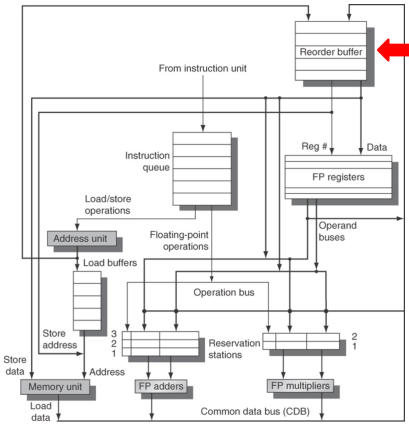
\includegraphics[scale = 0.5]{images/speculative-tomasulo}
    \caption{Speculative tomasulo}
    \label{fig:speculative-tomasulo}
\end{figure}

\subsubsection{ROB entries}
Each ROB entries contains four fields:
\begin{description}
    \item[Instruction type field] indicates whether instruction
    is a branch (no destination result), a store (has
    memory address destination), or a load/ALU
    (register destination)
    \item[Destination field] supplies register number (for
    loads and ALU instructions) or memory address (for
    stores) where results should be written
    \item[Value field] holds value of result until
    instruction commits
    \item[Ready filed] indicates that instruction has
    completed execution, ready to commit
\end{description}

\subsubsection{ROB extension}
The addition of the reorder buffer introduces changes in tomasulo:
\begin{itemize}[noitemsep]
    \item ROB completely replaces store buffers
    \item renaming function of reservation stations completely replaced
    \item reservation stations now only queue operations (and operands) to FUs between issue and execution.
    \item results are tagged with ROB entry number rather than with RS number, ROB entry must be tracked in the
    reservation stations
    \item all instructions excluding incorrectly predicted branches (or incorrectly speculated loads) commit when
    reaching head of ROB
    \item when a incorrectly predicted branch reaches the head, ROB is flushed, execution restarts at correct
    successor of branch \textrightarrow speculative active are easily undone
    \item processor with ROB can dynamically speculate while maintaining a precise interrupt model
\end{itemize}


    %! Author = lazza
%! Date = 07/05/2022

\section{Explicit register renaming}\label{sec:register-renaming}
Tomasulo provides \textit{implicit} register renaming by the means of reservation stations or ROB\@.
Now we introduce \textit{explicit} register renaming: use a physical register file that is larger than the number of
registers specified by the ISA\@.

Idea: allocate a new physical destination register for every instruction that writes:
\begin{itemize}[noitemsep]
    \item removes WAW, WAR hazards
    \item allows out-of-order completion (like tomasulo)
    \item similar to SSA, Static Single Assignment transformation done the compiler
\end{itemize}

\paragraph{Mechanism} Keep a translation table:
\begin{itemize}[noitemsep]
    \item map ISA \textit{logical} register to physical register
    \item when a register is written, replace the map entry with new register from freelist
    \item physical register becomes free when not used by any active instructions
\end{itemize}

\paragraph{Unified physical register file}
\begin{itemize}
    \item rename all architectural (logical) registers into a single physical register file during decode, no register
    values read
    \item FUs read and write from single unified register file holding committed and temporary registers in execution
    \item commit only updates mapping of architectural register to physical register, no data movement
\end{itemize}

\paragraph{HW register renaming}
\begin{description}
    \item[Renaming map] simple data structure that supplies the physical register number of the register that
    currently corresponds to the requested architectural register
    \item[Instruction commit] update permanently the renaming table to indicate that the physical register holding
    the destination values corresponds to the actual architectural register
    \item[ROB] Use reorder buffer to enforce in-order commit
\end{description}

\subsection{Explicit renaming - Scoreboard}\label{subsec:explicit-renaming---scoreboard}
\subsubsection{Stages}
\begin{description}
    \item[Issue] decode instructions and check for structural hazards \textcolor{red}{and allocate new physical
    register for result}:
    \begin{itemize}[noitemsep]
        \item[-] instructions issued in program order (for hazard checking)
        \item[-] \textcolor{red}{don't issue if there are no free physical registers}
        \item[-] don't issue if there's a structural hazard
    \end{itemize}
    \item[Read operands] wait until there are no more hazards, then read operands.
    All real dependencies solved in this stage, since we wait for instructions to write data back.
    \item[Execution] operate on operands.
    The functional unit begins execution upon receiving operands.
    When the result is ready, it notifies the scoreboard.
    \item[Write result] finish execution
\end{description}
\textbf{Note:} \textcolor{red}{no check for WAR and WAW hazards.}

\subsection{Register renaming vs ROB}\label{subsec:register-renaming-vs-rob}
\begin{itemize}[noitemsep]
    \item[-] instruction commit simpler than with ROB
    \item[-] deallocating register more complex
    \item[-] dynamic mapping or architectural to physical registers complicates design and debugging.
\end{itemize}



    %! Author = lazza
%! Date = 07/05/2022
\section{ILP limits}\label{sec:ilp-limits}
\subsection{Superscalar}\label{subsec:superscalar}
Superscalar execution allows multiples-issue and out-of-order execution.
A superscalar processor can execute more than one instruction during a clock cycle by simultaneously
dispatching multiple instructions to different execution units on the processor.
It therefore allows more throughput than would otherwise be possible at a given clock rate.
Each execution unit is not a separate processor (or a core if the processor is a multicore processor), but an
execution resource within a single CPU such as an arithmetic logic unit.
In Flynn's taxonomy, a single-core superscalar processor is classified as an SISD processor, though a single-core
superscalar processor that supports short vector operations could be classified as SIMD (single instruction stream,
multiple data streams).
A multicore superscalar processor is classified as an MIMD processor (multiple instruction streams, multiple data streams).
While a superscalar CPU is typically also pipelined, superscalar and pipelining execution are considered different
performance enhancement techniques.
The former executes multiple instructions in parallel by using multiple execution units, whereas the latter executes
multiple instructions in the same execution unit in parallel by dividing the execution (instruction) unit into
different phases.

\paragraph{Key requirements}
\begin{description}
    \item[-] Fetching more instructions per clock cycle: no major problem provided the instruction cache can sustain
    the bandwidth and can manage more requests at the same time.
    \item[-] Decide on data and control dependencies: dynamic scheduling and dynamic branch prediction
\end{description}

\paragraph{Beyond CPI = 1} 
\begin{itemize}[noitemsep]
    \item issue multiple instruction per clock-cycle
    \item varying number of instruction per cycle (1 to 8)
    \item scheduled by the compiler or HW
\end{itemize}
\[CPI_{ideal} =\frac{1}{issue-width}\]


With single-issue ILP we can be reach an ideal CPI =~1.
With superscalar execution our \textit{ideal} CPI can decrease furthermore.

\subsection{Assumptions}\label{subsec:assumptions}
The ideal machine must have:
\begin{description}
    \item[Register renaming] infinite virtual registers and all WAW and WAR hazards are avoided
    \item[Branch prediction] perfect, no mispredictions
    \item[Jump prediction] all jumps perfectly predicted, machine with perfect speculation and an unbounded buffer of
    instructions available
    \item[Memory address alias analysis]\footnote{Alias analysis is a technique used to determine if a storage location may be accessed in more than one way} addresses are know and a store can be moved before a load provided the 
    addresses not equal 
    \item[One cycle latency for all instructions] unlimited number of instructions issued per clock cycle
\end{description}

\subsection{Limits on window size}\label{subsec:limits-on-window-size}
Dynamic analysis is necessary to approach
perfect branch prediction (impossible at compile
time!).
A perfect dynamic-scheduled CPU should:
\begin{itemize}[noitemsep]
    \item[-] Look arbitrarily far ahead to find set of instructions to
    issue, predict all branches perfectly
    \item[-] Rename all registers uses (no WAW, WAR hazards);
    \item[-] Determine whether there are data dependencies
    among instructions in the issue packet, rename if
    necessary
    \item[-] Determine if memory dependencies exist among
    issuing instructions, handle them
    \item[-] Provide enough replicated functional units to allow all
    ready instructions to issue.
\end{itemize}
Size affects the number of comparisons necessary to determine
RAW dependencies.
The number of comparisons to evaluate for data dependencies among n register-to-register
instructions in the issue phase is \(n^2 - n\).

    %! Author = lazza
%! Date = 28/05/2022

\section{Multiprocessors}\label{sec:multiprocessors}
Till now we considered single cores architectures and how to increase the ILP in(side) such architectures.

\begin{figure}[h]
    \centering
    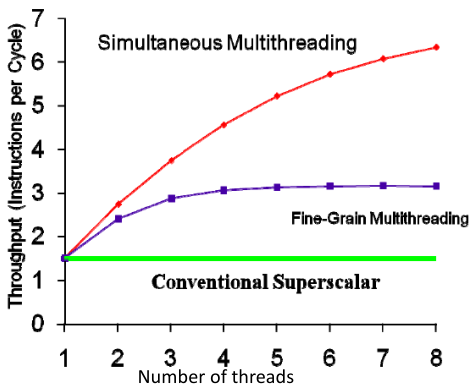
\includegraphics[scale = 0.4]{images/superscalar-vs-multithreading}
    \caption{Superscalar and multithreading}
    \label{fig:superscalar-and-multithreading}
\end{figure}

\paragraph{Beyond ILP}
We have seen the superscalar architecture, which can issue multiple instructions per clock cycle but these systems are
very complex to design and the returns are diminishing.
Another step forward towards parallelism is adding multithreading (or multiprocess) support to our single cores, but
the throughput of such systems reach their limits soon in terms of number of threads, what if we are willing to
have much more threads running?
Can we increase our throughput and support large-scale parallel systems?

\paragraph{Physical limitations}
\begin{itemize}
    \item difficult to increase performance and clock frequency of the single core
    \item a deep pipeline:
    \begin{itemize}
        \item heat dissipation
        \item speed light transmission problems in wires
        \item difficulties in design and verification
        \item requirement of very large design groups (higher complexity)
    \end{itemize}
\end{itemize}

Designing faster architectures may lead to worse throughput than running in parallel existing architectures;
furthermore, the design of a new architecture takes more time and cost.
Replication of cores doesn't come for free, to connect multiple microprocessor in a complex system we have to implement
some communication policies between cores.

\paragraph{Communication architecture} requires:
\begin{itemize}
    \item abstractions (HW/SW interfaces)
    \item different structures to realize abstraction efficiently
\end{itemize}

\subsection{Parallel architectures}\label{subsec:parallel-architecture}
\textit{“A parallel computer is a collection of
processing elements that cooperates and
communicate to solve large problems fast”}\footnote{Almasi and Gottlieb, Highly Parallel Computing, 1989}

Parallelism in hardware:
\begin{itemize}
    \item parallelism in a uniprocessor:
    \begin{itemize}
        \item pipelining
        \item superscalar, VLIM, etc.
    \end{itemize}
    \item SIMD instructions, vector processor, GPUs
    \item \textbf{multiprocessors}
\end{itemize}

\subsubsection{SISD}
A serial (non-parallel) computer with deterministic execution, i.e., the architectures seen till now, the oldest and
most common type of computer.
\begin{figure}[h]
    \centering
    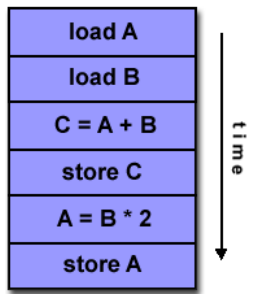
\includegraphics[scale = 0.3]{images/sisd}
    \caption{SISD}
    \label{fig:sisd}
\end{figure}

\subsubsection{MISD}
A parallel computer, where a single data stream is fed into multiple processing units.
Each processing unit operates on the data independently via independent instruction streams.
Niche use cases such as regex expressions.
\begin{figure}[H]
    \centering
    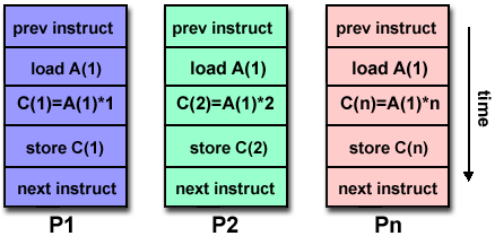
\includegraphics[scale = 0.3]{images/misd}
    \caption{MISD}
    \label{fig:misd}
\end{figure}

\subsubsection{SIMD}
A type of parallel computer, where all processing units execute the same instruction at any given clock cycle, each
one operates on a different data stream.
We have \textit{data pipelining} into processing unit -- e.g., useful for operations on matrices.
It is best suited for specialized problems characterized by a high degree of regularity, such as graphics/image
processing (GPUs) or machine learning.
SIMD processors are typically special-purpose.
There is only one single instruction memory and control processor to fetch and dispatch instructions.

\begin{figure}[H]
    \centering
    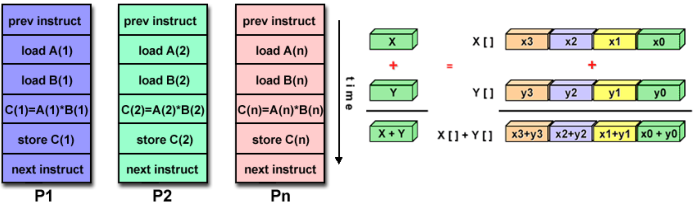
\includegraphics[scale = 0.3]{images/simd}
    \caption{SIMD}
    \label{fig:simd}
\end{figure}

A central controller broadcasts instructions to
multiple processing elements (PEs):
\begin{itemize}
    \item only requires one controller for whole array
    \item only requires storage for one copy of program
    \item all computations are fully synchronized
\end{itemize}

\begin{figure}[H]
    \centering
    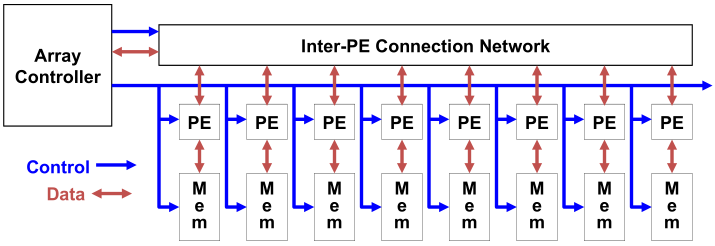
\includegraphics[scale = 0.3]{images/simd-scheme}
    \caption{SIMD scheme}
    \label{fig:simd-scheme}
\end{figure}

\begin{itemize}
    \item[\textrightarrow] Synchronized units: single Program Counter
    \item[\textrightarrow] Each unit has its own addressing registers\\
    – Can use different data addresses
    \item[\textrightarrow] Motivations for SIMD:\\
    – Cost of control unit shared by all execution units\\
    – Only one copy of the code in execution is necessary
    \item[\textrightarrow] Real life:\\
    – SIMD have a mix of SISD instructions and SIMD\\
    – A host computer executes sequential operations\\
    – SIMD instructions sent to all the execution units, which
    has its own memory and registers and exploit an
    interconnection network to exchange data
\end{itemize}

\paragraph{Alternative Model: Vector Processing}
Although being similar to SIMD, cannot be categorized under the Flynn's taxonomy.
SIMD instruction sets lack crucial features when compared to vector processor instruction sets, the most important of
these is that vector processors, inherently by definition and design, have always been variable-length since their
inception.

Vector processors have high-level operations that work on linear arrays of numbers: "vectors".
A vector processor consists of a pipelined scalar unit (may be out-of order or VLIW) plus a vector unit.

Styles of vector architectures:
\begin{itemize}
    \item \textit{memory-memory vector processors:} all vector
    operations are memory to memory
    \item \textit{vector-register processors:} all vector operations between vector registers (except load and store)
    , vector equivalent of load-store architectures
\end{itemize}

\begin{figure}[h]
    \centering
    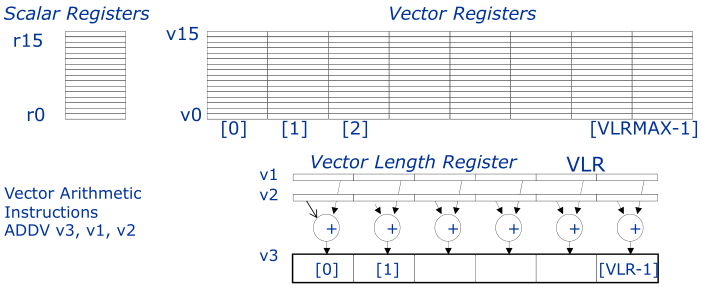
\includegraphics[scale = 0.35]{images/vector-programming-model}
    \caption{Vector programming model}
    \label{fig:vector-programming-model}
\end{figure}

\begin{table}[h]
    \begin{verbatim}
                # C code
                for (i=0;i<64; i++)
                C[i] = A[i]+B[i];
    \end{verbatim}
    \begin{tabular}{p{1.6in}|p{1.4in}}
        \begin{verbatim}
    # Scalar Code
    LI R4, #64
    loop:
    L.D F0, 0(R1)
    L.D F2, 0(R2)
    ADD.D F4, F2, F0
    S.D F4, 0(R3)
    DADDIU R1, 8
    DADDIU R2, 8
    DADDIU R3, 8
    DSUBIU R4, 1
    BNEZ R4, loop
        \end{verbatim} &
        \begin{verbatim}
    # Vector Code
    LI VLR, #64
    LV V1, R1
    LV V2, R2
    ADDV.D V3,V1,V2
    SV V3, R3
        \end{verbatim}
    \end{tabular}
    \label{tab:vector-programming-comparison}
\end{table}

add stuff from slide +\\
vector registers, more area more cost and more energy\\
vector machina distance between functional units can be bottleneck, use 3d structure.\\
situation: tons of data that we want to study\\

\textbf{Sony Playstation 2000:} a system running in parallel a MIPS cpu for I/O together with parallel
vector processors for image pre-processing.
\begin{figure}[h]
    \centering
    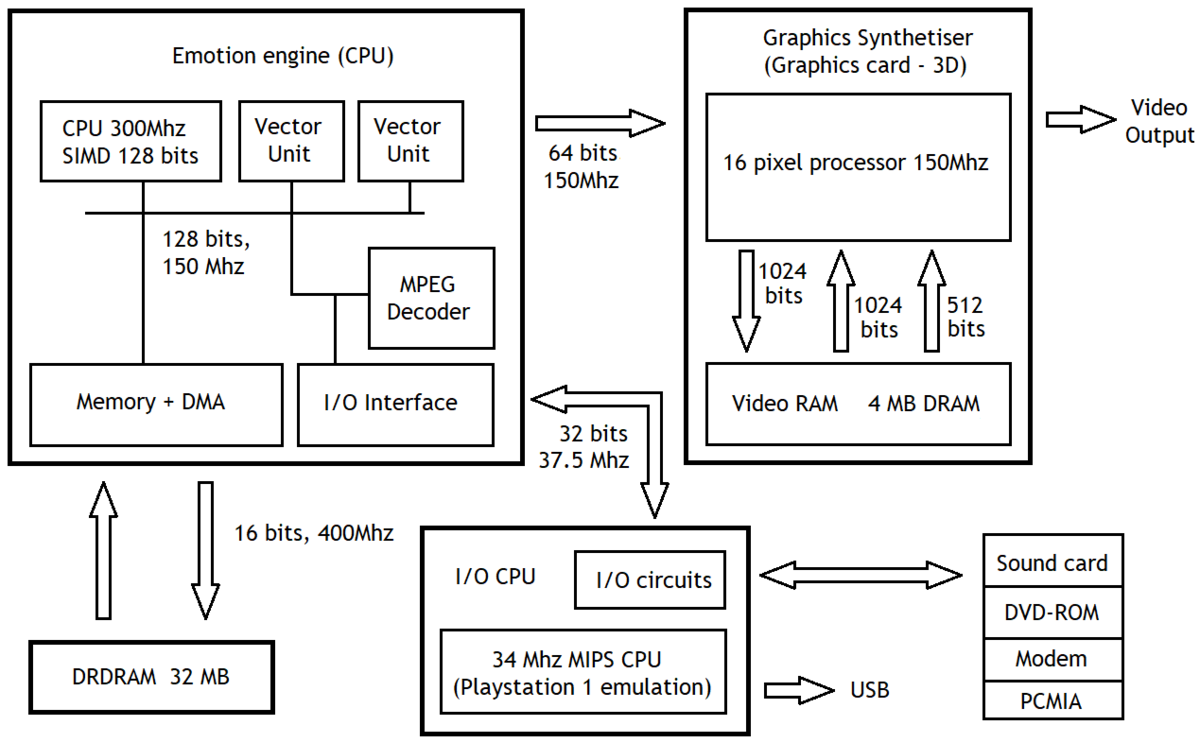
\includegraphics[scale = 0.2]{images/sony-playstation-2000}
    \caption{Sony Playstation 2000 architecture}
    \label{fig:sony-playstation}
\end{figure}

\subsubsection{MIMD}
The most common parallel computer nowadays, every processor may have a different instruction and data stream.
See chapter~\ref{sec:mimd}.

    %! Author = lazza
%! Date = 28/05/2022

\section{GPU}\label{sec:gpu}

\subsection{Procedural synthesis}\label{subsec:procedural-synthesis}
Procedural synthesis about making optimal use of system bandwidth
and main memory by dynamically generating lower-level geometry
data from statically stored higher-level scene data.

\begin{figure}[h]
    \centering
    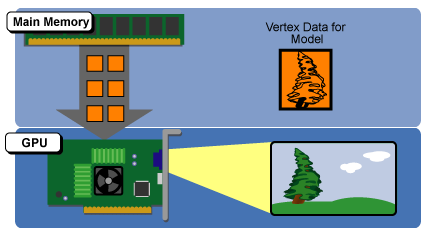
\includegraphics[width = \linewidth]{images/procedural-synthesis}
    \caption{Procedural synthesis}
    \label{fig:procedural-synthesis}
\end{figure}

For 3D games:
\begin{itemize}
    \item Artists use a 3D rendering program to produce content for the game
    \item Each model is translated into a collection of polygons
    \item Each polygons is represented in the computer's memory as collections of vertices
\end{itemize}
When the computer is rendering a scene in a game in real-time:
\begin{itemize}
    \item Models that are being displayed on the screen start out in main
memory as stored vertex data
    \item That vertex data is fed from main memory into the GPU where it is then rendered into a 3D image and output
    to the monitor as a sequence of frames.
\end{itemize}

\paragraph{Limitations} there are two problems:
\begin{itemize}
    \item The costs of creating art assets for a 3D game are
going through the roof along with the size and
complexity of the games themselves
    \item Console hardware's limited main memory sizes and
limited bus bandwidth
\end{itemize}

\paragraph{Xbox 360's solution}
Store high-level descriptions of objects in main memory.
Give the CPU the task of procedurally generate the geometry of the objects on the fly -- e.g., the vertex data are
generated by one or more running threads.
The GPU then takes the pre-processed vertex information and renders the tress normally, just as if it had gotten that
information from main memory.

\begin{figure}[h]
    \centering
    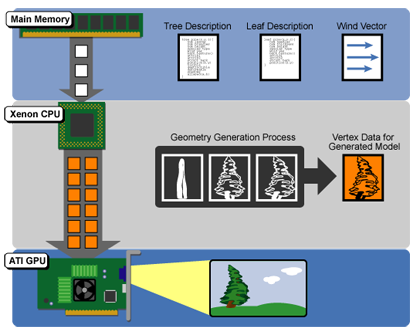
\includegraphics[width=\linewidth]{images/xbox-360-image-processing}
    \caption{Xbox 360 image processing}
    \label{fig:xbox-360-image-processing}
\end{figure}

\subsection{GPU vs CPU}\label{subsec:gpu-vs-cpu}
A GPU is tailored for high parallel operation while a
CPU executes programs serially.
For this reason, GPUs have many parallel execution
units and higher transistor counts, while CPUs have few
execution units and higher clock speeds.
A GPU is for the most part deterministic in its operation
(though this is quickly changing).
GPUs have much deeper pipelines (several thousand
stages vs 10--20 for CPUs).
GPUs have significantly faster and more advanced
memory interfaces as they need to shift around a lot
more data than CPUs.

\subsection{GPU pipeline}\label{subsec:gpu-pipeline}
The GPU receives geometry information from the CPU as an input and provides a picture as an output.
The five stages are:
\begin{itemize}
    \item host interface
    \item vertex processing
    \item triangle setup
    \item pixel processing
    \item memory interface
\end{itemize}

\begin{figure}[h]
    \centering
    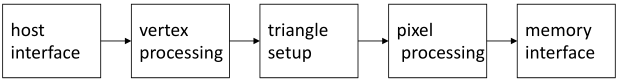
\includegraphics[width=\linewidth]{images/gpu-pipeline}
    \caption{GPU pipeline}
    \label{fig:gpu-pipeline}
\end{figure}

\subsubsection{Host interface}
The host interface is the communication bridge between the CPU and the GPU\@.
It receives commands from the CPU and also pulls geometry information from system memory.
It outputs a stream of vertices in object space with all their associated information (normals, texture
coordinates, per vertex color, etc.)

\subsubsection{Vertex processing}
The vertex processing stage receives vertices from the host interface in object space and outputs them in screen space.
This may be a simple linear transformation, or a complex operation involving morphing effects.
Normals, texcoords, etc., are also transformed.
No new vertices are created in this stage, and no vertices are discarded (input/output has 1:1 mapping).

\subsubsection{Triangle setup}
In this stage geometry information becomes raster information: screen space geometry is the input, pixels are the 
output.
Prior to rasterization, triangles that are back-facing or are located outside the viewing frustum are rejected.
Some GPUs also do some hidden surface removal at this stage.

\subsubsection{Fragment processing}
Each fragment provided by triangle setup is fed into fragment processing as a set of attributes (position, normal, 
textcoord, etc.), which are used to compute the final color for this pixel.
The computation taking place here include texture mapping and math operations.
Typically the bottleneck in modern applications.

\subsubsection{Memory interface}
Fragment colors provided by the previous stage are written to the framebuffer.
It used to be the biggest bottleneck before fragment processing took over.
Before final write occurs, some fragments are rejected by the zbuffer, stencil and alpha tests.
On modern GPUs, z and color are compressed to reduce framebuffer bandwidth (but not size).


\subsection{Programmability in the GPU}\label{subsec:programmability-in-the-gpu}
Vertex and fragment processing, and now triangle set-up, are programmable.
The programmer can write programs that are executed for every vertex as well as for every fragment.
This allows fully customizable geometry and shading effects that go well beyond the generic look and feel of old 3D
applications.

\begin{figure}[h]
    \centering
    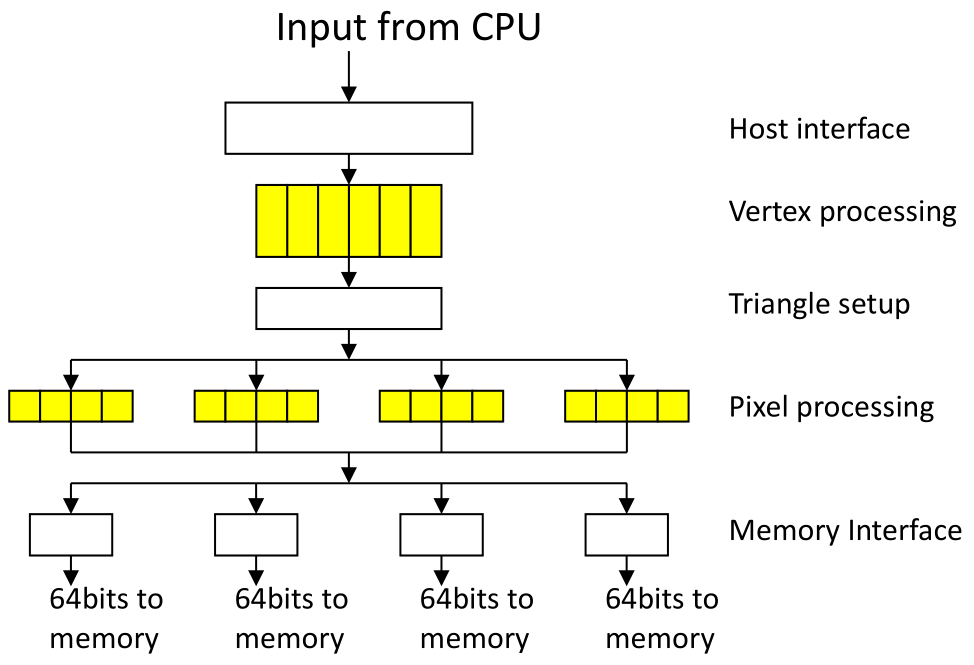
\includegraphics[width=\linewidth]{images/gpu-hierarchy}
    \caption{GPU pipeline}
    \label{fig:gpu-hierarchy}
\end{figure}

\subsection{Command buffer CPU-GPU}\label{subsec:command-buffer-cpu-gpu}
The CPU and GPU inside the \textit{heterogeneous} system work in parallel with each other.
There are two "threads" going on, one for the CPU and one for the GPU, which communicate through a command buffer:

\begin{figure}[h]
    \centering
    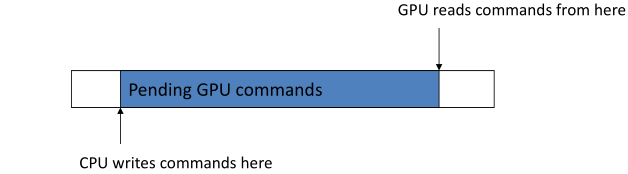
\includegraphics[width=\linewidth]{images/gpu-command-buffer}
    \caption{GPU command buffer}
    \label{fig:gpu-command-buffer}
\end{figure}

If this command buffer is drained empty, we are CPU limited and the GPU will spin around waiting for new input.
If the command buffer fills up, the CPU will spin around waiting for the GPU to consume it, and we are effectively
GPU limited.

Another important point to consider is that programs that use the GPU do not follow the traditional sequential
execution model.
In the CPU program below, the object is not drawn after statement A and before statement B:
\begin{center}
    \textbf{statement A}\\
    \textcolor{red}{\textbf{API call to draw object}}\\
    \textbf{statement B}
\end{center}

Instead, all the API call does, is to add the command to draw the object to the GPU command buffer.

\subsubsection{Synchronization issues}
\paragraph{Referring data}
In figure~\ref{fig:gpu-buffer-referring-data}, the CPU must not overwrite the data in the "yellow" block until the GPU
is done with the "black" command, which references that data.

\begin{figure}[h]
    \centering
    \includegraphics[width=\linewidth]{images/gpu-buffer-referring-data}
    \caption{Referring data}
    \label{fig:gpu-buffer-referring-data}
\end{figure}

Moderns APIs implement semaphore style operations to keep this from causing problems.
If the CPU attempts to modify a piece of data that is being referenced by a pending GPU command it will have to spin
around waiting, until the GPU is finished with that command.
While this ensures correct operation it is not good for
performance since there are a million other things we’d
rather do with the CPU instead of spinning.
The GPU will also drain a big part of the command
buffer thereby reducing its ability to run in parallel with
the CPU\@.

\paragraph{Inlining data}
One way to avoid these issues is to inline all data to the command buffer and avoid references to separate data:

\begin{figure}[h]
    \centering
    \includegraphics[width=\linewidth]{images/gpu-buffer-inlining-data}
    \caption{Inlining data}
    \label{fig:inlining-data}
\end{figure}

However, this is also bad for performance, since we
may need to copy several megabytes of data instead of
merely passing around a pointer.

\paragraph{Renaming data}
A better solution is to allocate a new data block and
initialize that one instead, the old block will be deleted
once the GPU is done with it.
Modern APIs do this automatically, provided you
initialize the entire block (if you only change a part of the
block, renaming cannot occur).

\begin{figure}[h]
    \centering
    \includegraphics[width=\linewidth]{images/gpu-buffer-renaming-data}
    \caption{Renaming data}
    \label{fig:gpu-buffer-renaming-data}
\end{figure}

Better yet, allocate all your data at startup and don’t
change them for the duration of execution (not always
possible, however).

\subsubsection{GPU read-backs}
The output of a GPU is a rendered image on the screen,
what will happen if the CPU tries to read it?
The GPU must be synchronized with the CPU, i.e., it
must drain its entire command buffer, and the CPU must
wait while this happens.
We lose all parallelism, since first the CPU waits for the
GPU, then the GPU waits for the CPU (because the
command buffer has been drained).
Both CPU and GPU performance take a nosedive.
\textbf{Bottom line:} the image the GPU produces is for your
eyes, not for the CPU (treat the CPU \textrightarrow GPU highway as
a one way street).

\subsubsection{GPU tips}
Since the GPU is highly parallel and deeply pipelined,
try to dispatch large batches with each drawing call.
Sending just one triangle at a time will not occupy all of
the GPU’s several vertex/pixel processors, nor will it fill
its deep pipelines.

Since all GPUs today use the zbuffer algorithm to do
hidden surface removal, rendering objects front-to-back
is faster than back-to-front (painters algorithm), or
random ordering.
Of course, there is no point in front-to-back sorting if you
are already CPU limited.

\paragraph{nVidea G80 GPU} Characteristics:\\
\textrightarrow 128 streaming floating point processors @1.5Ghz\\
\textrightarrow 1.5 Gb Shared RAM with 86Gb/s bandwidth\\
\textrightarrow 500 GFLOPS on one chip (single precision)

\begin{figure}[h]
    \centering
    \includegraphics[width=\linewidth]{images/cpu-vs-gpu-performance}
    \caption{CPU vs GPU comparison}
    \label{fig:cpu-vs-gpu-performance}
\end{figure}

\paragraph{Why are GPU's so fast?}
\begin{itemize}
    \item Entertainment Industry has driven the economy
    of these chips
    \item Moore’s Law ++
    \item Simplified design (stream processing)
    \item Single-chip designs.
\end{itemize}

\paragraph{Modern GPU} has more ALUSs, devoting more transistors to data processing.
\begin{figure}[h]
    \centering
    \includegraphics[width = \linewidth]{images/gpu-alu-s}
    \caption{ALUs in CPU vs GPU}
    \label{fig:gpu-alu-s}
\end{figure}

\textbf{Very efficient} for:
\begin{itemize}
    \item Fast Parallel Floating Point Processing
    \item Single Instruction Multiple Data Operations
    \item High Computation per Memory Access
\end{itemize}

\textbf{Not as efficient} for:
\begin{itemize}
    \item Double Precision
    \item Logical Operations on Integer Data
    \item Branching-Intensive Operations
    \item Random Access, Memory-Intensive Operations
\end{itemize}
    %! Author = lazza
%! Date = 28/05/2022

\section{MIMD}\label{sec:mimd}
The execution can be synchronous or asynchronous, deterministic or non-deterministic.

\paragraph{Advantages:} \textbf{Multipurpose} processor that can be built starting from \textbf{standard CPUs} (often
off-the-shelf
microprocessors) that act independently one from the other: each processor fetches its own instructions and operates
on its own data.
\textbf{Scalable} to a variable number of processor nodes.\\
\textbf{Flexible:}
\begin{itemize}
    \item single-user machines focusing on high-performance for one
    specific application
    \item multi-programmed machines running many tasks
    simultaneously
    \item some combination of these functions.
\end{itemize}
\textbf{Cost/performance} advantages due to the use of off-
the-shelf microprocessors these can be combined in the same system.

\paragraph{Disadvantage:} Fault tolerance issues.

\paragraph{Exploting MIMD} To exploit a MIMD with $n$ processors, we need:
\begin{itemize}
    \item at least $n$ threads or processes to execute
    \item independent threads typically identified by the programmer or
    created by the compiler
    \item parallelism is contained in the threads \textrightarrow thread-level parallelism
\end{itemize}

\textbf{Note:} parallelism is identified by the software.\\

\subsection{Memory architecture}\label{subsec:memory-architecture}
Existing MIMD machines fall into 2 classes, depending on the number
of processors involved, which in turn dictates a memory organization
and interconnection strategy.

\paragraph{Key design issues}
\begin{itemize}
    \item how many processors?
    \item how powerful are processors?
    \item how do parallel processors share data?
    \item where to place the physical memory?
    \item how do parallel processors cooperate and coordinate?
    \item what type of interconnection topology?
    \item how to program processors?
    \item how to maintain cache coherency?
    \item how to maintain memory consistency?
    \item how to evaluate system performance?
\end{itemize}

\subsubsection{Centralized shared-memory architectures}\label{subsubsec:centralized-shared-memory-architectures}
\begin{itemize}
    \item at most few dozen processor chips (< 100 cores)
    \item large caches, single memory multiple banks
    \item often called symmetric multiprocessors (SMP) and the
    style of architecture called Uniform Memory Access (UMA), see section~\ref{subsec:bus-based-symmetric-shared-memory}
\end{itemize}

\begin{figure}[h]
    \centering
    \includegraphics[scale = 0.2]{images/centralized-shared-memory-architectures}
    \caption{Shared memory architecture}
    \label{fig:centralized-shared-memory-architectures}
\end{figure}

\subsubsection{Distributed memory architectures}\label{subsubsec:distributed-memory-architectures}
\begin{itemize}
    \item to support large processor counts
    \item requires high-bandwidth interconnect
    \item disadvantage: need of data communication among processors
    \item Non Uniform Memory Access (NUMA)
\end{itemize}

\begin{figure}[h]
    \centering
    \includegraphics[scale = 0.2]{images/distributed-memory-architectures}
    \caption{Distributed memory architectures}
    \label{fig:distributed-memory-architectures}
\end{figure}

\paragraph{Tile64} is a VLIW ISA multicore processor manufactured by Tilera.
It consists of a mesh network of 64 "tiles", where each tile houses a general purpose processor, cache,
and a non-blocking router, which the tile uses to communicate with the other tiles on the processor.
The short-pipeline, in-order, three-issue cores implement a MIPS-inspired VLIW instruction set.
Each core has a register file and three functional units: two integer arithmetic logic units and a load-store unit.
Each of the cores ("tile") has its own L1 and L2 caches plus an overall virtual L3 cache which is an aggregate of all
the L2 caches.
A core is able to run a full operating system on its own or multiple cores can be used to run a symmetrical
multi-processing operating system.

\begin{figure}[h]
    \centering
    \includegraphics[scale = 0.4]{images/Tile64}
    \includegraphics[scale = 0.5]{images/Tile64-Tile}
    \caption{Tile64}
    \label{fig:tile64}
\end{figure}


\subsubsection{Examples}\label{subsubsec:examples}

\paragraph{Cell: PS3}
Cell is a heterogeneous chip multiprocessor:
\begin{itemize}
    \item One 64-bit Power core
    \item 8 specialized co-processors\\
    \textrightarrow based on a novel single-instruction multiple-data (SIMD)
    architecture called SPU (Synergistic Processor Unit)
\end{itemize}

\paragraph{Xenon: XBOX360}
Xenon is a homogeneous chip multiprocessor:
\begin{itemize}
    \item three symmetrical cores, each two way SMT-capable and clocked at 3.2 GHz
    \item SIMD: VMX128 extension for each core
    \item 1 MMB L2 cache (lockable by the GPU) running at half-speed (1.6 GHz) with a 256-bit bus
\end{itemize}

Microsoft envisions a procedurally rendered game
as having at least two primary components:
\begin{itemize}
    \item Host thread: a game's host thread will contain the main
thread of execution for the game
    \item Data generation thread: where the actual procedural
synthesis of object geometry takes place
\end{itemize}
These two threads could run on the same PPE, or
they could run on two separate PPEs.
In addition to the these two threads, the game
could make use of separate threads for handling
physics, artificial intelligence, player input, etc.


\subsection{Procedural synthesis}\label{subsec:procedural-synthesis}
Procedural synthesis about making optimal use of system bandwidth
and main memory by dynamically generating lower-level geometry
data from statically stored higher-level scene data.

\begin{figure}[h]
    \centering
    \includegraphics[width = \linewidth]{images/procedural-synthesis}
    \caption{Procedural synthesis}
    \label{fig:procedural-synthesis}
\end{figure}

For 3D games:
\begin{itemize}
    \item Artists use a 3D rendering program to produce content for the game
    \item Each model is translated into a collection of polygons
    \item Each polygons is represented in the computer's memory as collections of vertices
\end{itemize}
When the computer is rendering a scene in a game in real-time:
\begin{itemize}
    \item Models that are being displayed on the screen start out in main
memory as stored vertex data
    \item That vertex data is fed from main memory into the GPU where it is then rendered into a 3D image and output
    to the monitor as a sequence of frames.
\end{itemize}

\paragraph{Limitations} there are two problems:
\begin{itemize}
    \item The costs of creating art assets for a 3D game are
going through the roof along with the size and
complexity of the games themselves
    \item Console hardware's limited main memory sizes and
limited bus bandwidth
\end{itemize}


\subsection{Memory Address Space Model}\label{subsec:memory-address-space-model}
How do parallel processors share data?
We already talked about how the physical memory implementation divides the \textit{machines} in two classes, now we 
look how the virtual memory is from the perspective of a process.

\subsubsection{Single logically shared address space}
A memory reference can be made by any processor to any memory location, this model adapts well to the
\textit{shared memory architectures}: the address space is shared among processors, the same physical address on 2
processors refers to the same location in memory.

\begin{figure}[h]
    \centering
    \includegraphics[scale = 0.3]{images/single-logically-shared-address-space}
    \caption{Single logically shared address space}
    \label{fig:single-logically-shared-address-space}
\end{figure}

\paragraph{Shared Address}
\begin{itemize}
    \item the processors communicate among them through shared variables in memory
    \item implicit management of the communication through load/store operations to access any memory locations
    \item shared memory does not mean that there is a single centralized memory
\end{itemize}

\subsubsection{Multiple and private address spaces}
The processors communicate among them through send/receive primitives, this model adapts well to \textit{message
passing architectures}: the address space is logically disjoint and cannot be addressed by different processors, the
same physical address on 2 processors refers to 2 different locations in two different memories.

\begin{figure}[h]
    \centering
    \includegraphics[scale = 0.3]{images/multiple-and-private-address-spaces}
    \caption{Multiple and private address spaces}
    \label{fig:multiple-and-private-address-spaces}
\end{figure}

\paragraph{Private address}
\begin{itemize}
    \item the processors communicate among them through sending/receiving messages
    \item explicit management of the communication through send/receive primitives to access private memory locations
    \item no cache coherency problem among processors
\end{itemize}

\textbf{Note:} The concepts of addressing space
(single/multiple) and the physical memory
organization (centralized/distributed) are
orthogonal to each other: they could be combined freely.
Multiprocessor systems can have single
addressing space and distributed physical
memory.

\begin{figure}[h]
    \centering
    \includegraphics[scale = 0.43]{images/address-space-vs-physical-memory-org}
    \caption{Single shared space vs physical memory}
    \includegraphics[scale = 0.40]{images/address-space-vs-physical-memory-org-1}
    \caption{Multiple private addresses vs physical memory }
    \label{fig:address-space-vs-physical-memory-org}
\end{figure}


\subsection{Programming Model}\label{subsec:programming-model}

\subsubsection{Shared Memory}
The program is a collection of threads of control, each thread:
\begin{itemize}
    \item can be created dynamically, mid execution, in some languages.
    \item has a set of \textit{private} variables, e.g., local stack variables
    \item also a set of \textit{shared} variables, e.g., static variables, shared common blocks, or global heap
\end{itemize}

Processes communication:
\begin{itemize}
    \item implicitly by writing and reading shared variables
    \item coordination by synchronizing on shared variables
\end{itemize}

\begin{figure}[h]
    \centering
    \includegraphics[width = \linewidth]{images/shared-memory-model}
    \caption{Shared memory}
    \label{fig:shared-memory-model}
\end{figure}

\paragraph{Advantages}
\begin{itemize}
    \item implicit communication (loads/stores)
    \item low overhead when cached
\end{itemize}

\paragraph{Disadvantages}
\begin{itemize}
    \item complex to build in way that scales well -- e.g., distance between core and memory may become too much
    cutting down performance
    \item requires synchronization operations
    \item hard to control data placement within caching system
\end{itemize}

\subsubsection{Message Passing}
The program consist of a collection of \textbf{named} processes:
\begin{itemize}
    \item usually fixed at program startup time
    \item thread of control plus local address space, no shared data
    \item logically shared data is partitioned over local processes
\end{itemize}

Processes communication:
\begin{itemize}
    \item explicitly by send/receive pairs
    \item coordination is implicit in every communication event
    \item MPI (Message Passing Interface) is the most commonly used SW
\end{itemize}

\begin{figure}[h]
    \centering
    \includegraphics[width = \linewidth]{images/message-passing-model}
    \caption{Message passing}
    \label{fig:message-passing-model}
\end{figure}

\paragraph{Advantages}
\begin{itemize}
    \item explicit communication (sending/receiving of messages)
    \item easier to control data placement (no automatic caching)
\end{itemize}

\paragraph{Disadvantages}
\begin{itemize}
    \item message passing overhead can be quite high
    \item more complex to program
    \item introduces question of reception technique (interrupts/polling)
\end{itemize}

\paragraph{Massively Parallel Processors Problems}
\begin{itemize}
    \item all data must be handled by software: cannot retrieve remote data except with message request/reply
    \item message passing has high software overhead:
    \begin{itemize}
        \item early machines had to invoke OS on each message
        \item even user level access to network interface has dozens of cycle overhead
        \item sending messages can be cheap (just like stores)
        \item receiving messages is expensive, need to poll or interrupt
    \end{itemize}
\end{itemize}

\subsection{Bus-based symmetric shared memory}\label{subsec:bus-based-symmetric-shared-memory}
The most popular architecture till now sees each core and its own cache memory, with a simple networking solution, the
bus, which connects processors with each other and to the shared memory.

\textbf{Note:} here we refer to \textit{physical} shared memory architecture (UMA).

\begin{figure}[h]
    \centering
    \includegraphics[scale = 0.45]{images/bus-based-symmetric-shared-memory}
    \caption{Bus-based symmetric multiprocecessors}
    \label{fig:bus-based-symmetric-shared-memory}
\end{figure}

Attractive as throughput servers and for parallel programs:
\begin{itemize}
    \item Fine-grain resource sharing
    \item Uniform access via loads/stores
    \item Automatic data movement and coherent replication in caches
    \item Cheap and powerful extension
\end{itemize}
It uses the normal uni-processor mechanisms to access data, the key to make it viable is the extension of memory
hierarchy to support multiple processors.

\paragraph{Shared memory machines} Two main categories:
\begin{itemize}
    \item non cache coherent
    \item hardware cache coherent
\end{itemize}
Will work with any data, but might be slow, we can choose to optimize only critical portions of code.
Load and store instructions used to communicate data: no OS involvement \textrightarrow low software overhead.
Usually there are some special synchronization primitives.
In large scale systems, the logically distributed shared memory is implemented as physically distributed memory
modules.\footnote{Some notions might be wrong in this section, double check}

\subsection{Cache coherence}\label{subsec:cache-coherence}
Shared memory architectures cache both \textbf{private data}, used by a single processor, and \textbf{shared data},
used by multiple processors to provide communication.
When shared data is cached, the shared valued may be replicated in multiple caches.
In addition to the reduction in access latency and required memory bandwidth, this replication provides a reduction
of shared data contention when multiple processors have to read simultaneously the same data.
Private processors caches create a problem:
\begin{itemize}
    \item copies of a variable can be present in multiple caches
    \item a write by one processor may not become visible to others
\end{itemize}
The use of multiple copies of the same data introduces a new problem: cache coherency.

\paragraph{Writing policies}
When a system writes data to cache, it must at some point write that data to the backing store as well.
The timing of this write is controlled by what is known as the write policy.
There are two basic writing approaches:
\begin{itemize}
    \item \textbf{write-through}: write is done synchronously both to the cache and to the backing store
    \item \textbf{write-back} (also called write-behind): initially, writing is done only to the cache.
    The write to the backing store is postponed until the modified content is about to be replaced by another cache block.
\end{itemize}

\begin{figure}[h]
    \centering
    \includegraphics[scale = 0.4]{images/cache-coherence-problem}
    \caption{Cache coherence problem}
    \label{fig:cache-coherence-problem}
\end{figure}
\textbf{Note:} processors see different values for $u$ after event 3.
With write back caches, the value written back to memory depends on which cache flushes or writes back values first:
processes accessing main memory may see very stale value.

\paragraph{What does coherency means}
Informal definition: \textit{"any read must return the most recent write} \textrightarrow too strict and difficult to
implement.\\
A better definition: \textit{any write must eventually be seen by a read}, all write are seen in \textbf{serialized
order}, that is two write to the same location by any two processors are seen in the same order by all processors
plus the latest (in time) will be seen (in memory).
If P writes x and P1 reads it, P’s write will be seen by P1 if the read
and write are sufficiently far apart and no other writes to x occur
between the two accesses: \textbf{propagation of writes} after a certain amount of time.

\paragraph{When a written value will be seen?}
We cannot require that a read of x by P1 can
instantaneously see the write of x by another
processor that precedes by a small amount of time.
This is a problem of \textbf{memory consistency}, coherency and consistency are complementary:
\begin{itemize}
    \item coherence defines the behavior of reads and writes to the same memory location
    \item consistency defines the behavior of reads and write with respect to accesses to other memory locations
\end{itemize}
Assumptions for now:
\begin{itemize}
    \item a write does not complete (and allow the next write to occur) until all processors have seen the effect of
    that write
    \item the processor does not change the order of any write with respect to any other memory access
\end{itemize}

\paragraph{Coherent caches}
A program running on multiple processors will normally
have copies of the same data in several caches.
In a coherent multiprocessor the caches provide both
\textbf{migration} and \textbf{replication} of shared data items:
\begin{itemize}
    \item Migration: a data item can be moved to a local cache
    and used there in a transparent fashion, reduces both the latency to access a shared data item that
    is allocated remotely and the \textit{bandwidth demand} on the shared memory
    \item Replication for shared data that are being
    simultaneously read: caches make a copy of the data
    item in the local cache, reduces both latency of access and \textit{contention for a shared read}
\end{itemize}

\paragraph{Potential solutions} HW-based solutions to maintain coherency: cache-coherence protocols.
Key issue: implement a cache coherent protocol in multiprocessors needs tracking the status of any sharing of a data
block.
Two classes of protocols:
\begin{itemize}
    \item snooping protocols
    \item directory-based protocols
\end{itemize}


\subsubsection{Snooping Protocols}
\begin{itemize}
    \item[\textrightarrow] All cache controllers monitor (snoop) on the bus to
    determine whether or not they have a copy of the block
    requested on the bus and respond accordingly.
    \item[\textrightarrow] Every cache that has a copy of the shared block, also
    has a copy of the sharing status of the block, and no
    centralized state is kept.
    \item[\textrightarrow]
    Send all requests for shared data to all processors.
    \item [\textrightarrow] Require broadcast, since caching info is at processors.
    \item [\textrightarrow] Suitable for Centralized Shared-Memory Architectures,
    and in particular for small scale multiprocessors with
    single shared bus.
\end{itemize}

\paragraph{Snoopy cache Goodman 1983}
Idea: have cache watch (or snoop upon) DMA\footnote{Direct Memory Access}, and then \textit{do the right thing}.
Snoopy caches tags are dual-ported:

\begin{figure}[h]
    \centering
    \includegraphics[scale = 0.4]{images/snoopy-cache-goodman}
    \caption{Snoopy cache goodman}
    \label{fig:snoopy-cache-goodman}
\end{figure}

Bus is a broadcast medium and caches know what
they have.
Cache controller “snoops” all transactions on the
shared bus:
\begin{itemize}
    \item relevant transaction if the cache contains that block
    \item take action to ensure coherence (\textrightarrow invalidate, update, or supply value):
    \subitem depends on state of the block and the protocol
\end{itemize}

\begin{figure}[h]
    \centering
    \includegraphics[width=\linewidth]{images/cache-snooping-protocol}
    \caption{Cache snooping}
    \label{fig:cache-snooping}
\end{figure}

Since every bus transaction checks the cache
address tags, this checking can interfere with the
processor operations.
When there is interference, the processor will likely
stall because the cache is unavailable.
To reduce the interference with the processor’s
accesses to the cache, we duplicate the address
tag portion of the cache (not the whole cache) for
snooping activities.
In practice, an extra read port is added to the
address tag portion of the cache, hence the dual-ported cache.

\begin{figure}[h]
    \centering
    \includegraphics[width=\linewidth]{images/dual-ported-cache}
    \caption{Dual-ported cache}
    \label{fig:dual-ported-cache}
\end{figure}

\paragraph{Types of snooping protocols}
Snooping Protocols are of two types depending
on what happens on a write operation:
\begin{itemize}
    \item Write-Invalidate Protocol
    \item Write-Update or Write-Broadcast Protocol
\end{itemize}

\subsubsection{Write-invalidate Protocol}
The writing processor issues an invalidation signal
over the bus to cause all copies in other caches to
be invalidated before changing its local copy.
The writing processor is then free to update the
local data until another processor asks for it.
All caches on the bus check to see if they have a
copy of the data and, if so, they must invalidate the
block containing the data.
This scheme allows multiple readers but only a
single writer.
This scheme uses the bus only on the first write
to invalidate the other copies.
Use bus itself to serialize: write cannot complete until bus access is obtained
Subsequent writes do not result in bus activity.
This protocol provides similar benefits to write-
back protocols in terms of reducing demands
on bus bandwidth.
Read Miss: snoop in caches to find the most
recent copy.

\subsubsection{Write-update Protocol}
The writing processor broadcasts the new data over
the bus;
all caches check if they have a copy of the
data and, if so, all copies are updated with the new
value.
This scheme requires the continuous broadcast of
writes to shared data (while write-invalidate deletes
all other copies so that there is only one local copy
for subsequent writes).
This protocol is like write-through because all writes
go over the bus to update copies of the shared
data.
This protocol has the advantage of making the new
values appear in caches sooner \textrightarrow reduced latency.
Read Miss: memory always up-to-date.

\textbf{Note:} writing policies and snooping protocols are orthogonal concepts: a policy -- e.g, write back --
can be combined with any of the two snooping protocols.
The latter is about cache coherence the former about when to schedule writing transitions.

\subsubsection{Update vs Invalidate}
Question about program behavior: is a block written by one processor later read by others before it is overwritten?
\begin{table}[h]
    \centering
    \begin{tabular}{l|p{0.37\linewidth}p{0.37\linewidth}}
        \toprule
         & \textbf{Invalidate} & \textbf{Update} \\
        \midrule
        yes & readers will take a miss & avoids misses on later references \\
        \midrule
        no & multiple writes without additional traffic, also clears out copies that will never be used again &
        multiple useless updates \\
        \bottomrule
    \end{tabular}
    \caption{Update vs Invalidate}
    \label{tab:update-vs-invalidate}
\end{table}
For a better performance we need to look at program reference patterns and hardware complexity.

Most part of commercial cache-based
multiprocessors uses:
\begin{itemize}
    \item Write-Back Caches to reduce bus traffic and
allow more processors on a single bus.
    \item Write-Invalidate Protocol to preserve bus
bandwidth
\end{itemize}

The write serialization still due to bus serializing request: a write to a shared data item cannot actually
complete until it obtains bus access.

\paragraph{Write back cache}
How to identify the most recent data value of a cache block in case of cache miss?
It could be in (another) cache or in memory.
We use the same snooping scheme both for cache misses and writes:
\begin{itemize}
    \item each processor snoops every address placed on the bus
    \item if a processor finds that it has a dirty copy of the
    requested cache block, it provides the cache block
    in response to the read request
    \item memory access is aborted
\end{itemize}

\paragraph{Write back cache, write invalidate}
Each \textit{block of memory} is in one of three states:
\begin{itemize}
    \item \textbf{Clean} in all cache and up-to-date in memory (shared)
    \item \textbf{Dirty} in exactly one cache (exclusive)
    \item not in any caches
\end{itemize}
Each \textit{cache block} can be in one of three states:
\begin{itemize}
    \item \textbf{Clean} (or shared)(read only): the block is clean, not modified, and can be read
    \item \textbf{Dirty} (or modified or Exclusive): cache has only copy, its writeable, and dirty (block cannot be
    shared)
    \item \textbf{Invalid}: block contains no valid data
\end{itemize}

\paragraph{MSI invalidate protocol}
Three states:
\begin{itemize}
    \item \textbf{M}: "Modified"
    \item \textbf{S}: "Shared"
    \item \textbf{I}: "Invalid"
\end{itemize}
Read (\textit{PrRd}) obtains block in \textit{shared}, even if there is only the cache copy.\\
Before writing a process must obtain exclusive ownership:
\begin{itemize}
    \item \textit{BusRdx} causes others to invalidate (demote)
    \item if M in another cache, it will flush
    \item we need to send \textit{BusRdx} even if hit is in S (promote to M -- upgrade)
\end{itemize}
What about replacement?
S \textrightarrow I, M\textrightarrow I\@.
\begin{figure}[h]
    \centering
    \includegraphics[width=0.7\linewidth]{images/msi-protocol}
    \caption{MSI protocol}
    \label{fig:msi-protocol}
\end{figure}

\paragraph{Complications for the basic MSI protocol}
Operations (detect a miss, acquire bus, receive a response) are not atomic: creates the possibility of deadlock and
races.
One solution would be the processors that send the invalidate can hold the bus until other processors receive the
invalidate.

\paragraph{MESI write-invalidate protocol}
To prevent the need to write invalidate on a write we can add an exclusive state to indicate that the clean block is
in only one cache (owned state).
Each cache block can be in four states:
\begin{itemize}
    \item \textbf{Modified:} the block is dirty and cannot be shared, the cache has only copy, its writable
    \item \textbf{Exclusive:} the block is clean and cache has only copy
    \item \textbf{Shared:} the block is clean and other copies of the block are in cache
    \item \textbf{Invalid:} block contains no valid data
\end{itemize}
The exclusive state lets us distinguish between exclusive (writable) and owned (written).

\begin{figure}[h]
    \centering
    \includegraphics[width=\linewidth]{images/mesi-protocol-states}
    \caption{MESI states}
    \label{fig:mesi-protocol-states}
\end{figure}

\begin{figure}[h]
    \centering
    \includegraphics[width=0.7\linewidth]{images/mesi-protocol}
    \caption{MESI protocol}
    \label{fig:mesi-protocol}
\end{figure}

\textit{BusRd(S)} means shared line asserted on BusRd transaction.
Flush if there is a cache-to-cache transfer: only one cache flushes data.
Replacement:
S\textrightarrow I can happen
without telling other
caches, E \textrightarrow I, M\textrightarrow I\@.\\
In both S and E, the memory has an up-to-date
version of the data.
A write to a E block does not require to send the
invalidation signal on the bus, since no other
copies of the block are in cache.
A write to a S block implies the invalidation of
the other copies of the block in cache.

\begin{figure}[h]
    \centering
    \includegraphics[width=\linewidth]{images/mesi-automata}
    \caption{MESI automaton}
    \label{fig:mesi-automaton}
\end{figure}
\end{document}
